%-----------------------------------------------------------------------------
%
%               Template for sigplanconf LaTeX Class
%
% Name:         sigplanconf-template.tex
%
% Purpose:      A template for sigplanconf.cls, which is a LaTeX 2e class
%               file for SIGPLAN conference proceedings.
%
% Author:       Paul C. Anagnostopoulos
%               Windfall Software
%               978 371-2316
%               paul@windfall.com
%
% Created:      15 February 2005
%
%-----------------------------------------------------------------------------


\documentclass{sigplanconf}

% The following \documentclass options may be useful:
%
% 10pt          To set in 10-point type instead of 9-point.
% 11pt          To set in 11-point type instead of 9-point.
% authoryear    To obtain author/year citation style instead of numeric.

\usepackage{amsmath}
\usepackage[dvips]{graphicx}
\DeclareGraphicsExtensions{.eps, .ps}
\usepackage[caption=false,font=footnotesize]{subfig}
\usepackage{url}
\usepackage{listings}
\lstset{ %
language=Python,                % choose the language of the code
basicstyle=\ttfamily\footnotesize,  % the size of the fonts that are used for the code
keywordstyle=\bfseries,
frame=single,	                % adds a frame around the code
tabsize=4,   	                % sets default tabsize to 2 spaces
captionpos=b,                   % sets the caption-position to bottom
breaklines=true,                % sets automatic line breaking
breakatwhitespace=false,        % sets if automatic breaks should only happen at whitespace
escapeinside={\%*}{*)},          % if you want to add a comment within your code
xleftmargin=5mm,                % indent listing slightly to get line numbers back onto page
xrightmargin=5mm,
numbers=left, numberstyle=\ttfamily\bfseries\footnotesize
}

% correct bad hyphenation here
\hyphenation{Dist-Num-Py Glo-bal}

\begin{document}

\conferenceinfo{PGAS'10}{Oct 12--15, 2010, New York.} 
\copyrightyear{2010} 
%\copyrightdata{[to be supplied]}

%\titlebanner{DistNumPy}        % These are ignored unless
\preprintfooter{DistNumPy}   % 'preprint' option specified.

\title{Numerical Python for Scalable Architectures}

\authorinfo{Mads Ruben Burgdorff Kristensen \\ Brian Vinter}
           {eScience Centre\\ University of Copenhagen\\ Denmark}
           {madsbk@diku.dk/vinter@diku.dk}

\maketitle

\begin{abstract}
In this paper, we introduce DistNumPy, a library for doing numerical computation in Python that targets scalable distributed memory architectures. DistNumPy extends the NumPy module\cite{numpy}, which is popular for scientific programming. Replacing NumPy with DistNumPy enables the user to write sequential Python programs that seamlessly utilize distributed memory architectures. This feature is obtained by introducing a new backend for NumPy arrays, which distribute data amongst the nodes in a distributed memory multi-processor. All operations on this new array will seek to utilize all available processors. The array itself is distributed between multiple processors in order to support larger arrays than a single node can hold in memory. 

We perform three experiments of sequential Python programs running on an Ethernet based cluster of SMP-nodes with a total of 64 CPU-cores. The results show an 88\% CPU utilization when running a Monte Carlo simulation, 63\% CPU utilization on an N-body simulation and a more modest 50\% on a Jacobi solver. The primary limitation in CPU utilization is identified as SMP limitations and not the distribution aspect. Based on the experiments we find that it is possible to obtain significant speedup from using our new array-backend without changing the original Python code.
\end{abstract}

%\category{CR-number}{subcategory}{third-level}

%\terms
%term1, term2

\keywords
NumPy, Productivity, Parallel language

\section{Introduction}
In many scientific and engineering areas, there is a need to solve numerical problems. Researchers and engineers behind these applications often prefer a high level programming language to implement new algorithms. Of particular interest are languages that support a broad range of high-level operations directly on vectors and matrices. Also of interest is the possibility to get immediate feedback when experimenting with an application. The programming language Python combined with the numerical library NumPy\cite{numpy} supports all these features and has become a popular numerical framework amongst researchers. 

The idea in NumPy is to provide a numerical extension to the Python language. NumPy provides not only an API to standardized numerical solvers, but a possibility to develop new numerical solvers that are both implemented and efficiently executed in Python, much like the idea behind the MATLAB\cite{guide1998mathworks} framework. 

NumPy is mostly implemented in C and introduces a flexible N-dimensional array object that supports a broad range of numerical operations. The performance of NumPy is significantly increased when using array-operations instead of scalar-operations on this new array.

Parallel execution is supported by a limited set of NumPy functions, but only in a shared memory environment. However, many scientific computations are executed on large distributed memory machines because of the computation and memory requirements of the applications. In such cases, the communication between processors has to be implemented by the programmer explicitly. The result is a significant difference between the sequential program and the parallelized program. DistNumPy eliminates this difference by introducing a distributed version of the N-dimensional array object. All operations on such distributed arrays will utilize all available processors and the array itself is distributed between multiple processors, which makes it possible to expand the size of the array to the aggregated available memory.

\subsection{Motivation}
\begin{figure}%
  \begin{center}%
    \subfloat[\label{fig:workflow1}]{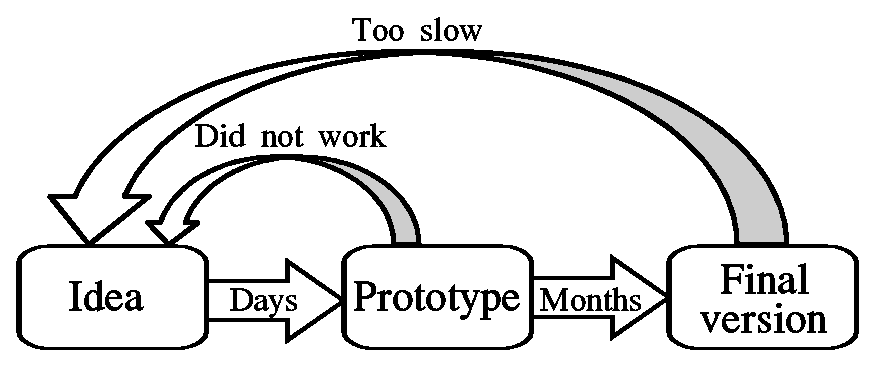
\includegraphics[width=170px]{gfx/workflow1}}
    \qquad
    \subfloat[\label{fig:workflow2}]{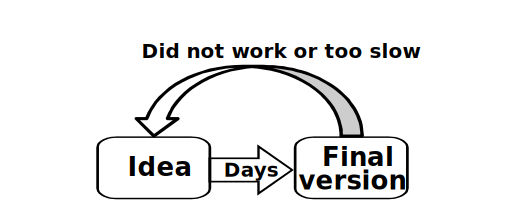
\includegraphics[width=170px]{gfx/workflow2}}
    \caption{Development workflow. (a) is a typical workflow that involves two languages: one for the prototype and one for the final version. In (b) only one language is used in the workflow.
    }%
    \label{fig:workflow}%
  \end{center}
\end{figure}

Solutions to numerical problems often consist of two implementations: a prototype and a final version. The algorithm is developed and implemented in a prototype by which the correctness of the algorithm can be verified. Typical many iterations of development are required to obtain a correct prototype, thus for this purpose a high productivity language is used, most often MATLAB. However, when the correct algorithm is finished the performance of the implementation becomes essential for doing research with the algorithm. This performance requirement presents a problem for the researcher since highly optimized code requires a fairly low-level programming language such as C/C++ or Fortran. The final version will therefore typical be a reimplementation of the prototype, which involves both changing the programming language and parallelizing the implementation (Fig. \ref{fig:workflow1}). 

The overall target of DistNumPy is to provide a high productivity tool that meets both the need for a high productivity tool that allows researcher to move from idea to prototype in a short time, and the need for a high performance solution that will eliminate the need for a costly and risky reimplementation (Fig. \ref{fig:workflow2}). It should be possible to develop and implement an algorithm using a simple notebook and then effortlessly execute the implementation on a cluster of computers while utilizing all available CPUs.


\subsection{Target architectures}
NumPy supports a long range of architectures from the widespread x86 to the specialized Blue Gene architecture. However, NumPy is incapable of utilizing distributed memory architectures like Blue Gene supercomputers or clusters of x86 machines. The target of DistNumPy is to close this gap and fully support and utilize distributed memory architectures. 


\subsection{Related work}
Libraries and programming languages that support parallelization on distributed memory architectures is a well known concept. The existing tools either seek to provide optimal performance in parallel applications or, like DistNumPy, seek to ease the task of writing parallel applications.

The library ScaLAPACK\cite{Blackford96} is a parallel version of the linear algebra library LAPACK\cite{lapack90}. It introduces efficient parallel operations on distributed matrices and vectors. To use ScaLAPACK, an application must be programmed using MPI\cite{mpi} and it is the responsibility of the programmer to ensure that the allocation of matrices and vectors comply with the distribution layout ScaLAPACK specifies.

Another library, Global Arrays\cite{Nieplocha96}, introduces a distributed data object (global array), which makes the data distribution transparent to the user. It also supports efficient parallel operations and provides a higher level of abstraction than ScaLAPACK. However, the programmer must still explicitly coordinate the multiple processes that are involved in the computation. The programmer must specify which region of a global array is relevant for a given process.

Both ScaLAPACK and Global Arrays may be used from within Python and can even be used in combination with NumPy, but it is only possible to use NumPy locally and not with distributed operations. A more closely integrated Python project IPython\cite{PER-GRA:2007} supports parallelized NumPy operations. IPython introduces a distributed NumPy array much like the distributed array that is introduced in this paper. Still, the user-application must use the MPI framework and the user has to differentiate between the running MPI-processes.

Co-Array Fortran\cite{Co-arrayFortran98} is a  small language extension of Fortran-95 for parallel processing on Distributed Memory Machines. It introduce a Partitioned Global Address Space (PGAS) by extending Fortran arrays with a \emph{co-array} dimension. Each process can access remote instances of an array by indexing into the co-array dimensions. A similar PGAS extension called Unified Parallel C (UPC)\cite{Carlson99_UPC} extent the C language with a distributed array declaration. Both languages provide a high abstraction level, but users still program with the SPMD model in mind, writing code with the understanding that multiple instances of it will be executing cooperatively.

A higher level of abstraction is found in projects where the execution, seen from the perspective of the user, is represented as a sequential algorithm. The High Performance Fortran (HPF)\cite{Loveman93} programming languages provide such an abstraction level. However, HPF requires the user to specify parallelizable regions in the code and which data distribution scheme the runtime should use.

The Simple Parallel R INTerface (SPRINT)\cite{Hill08} is a parallel framework for the programming language R. The abstraction level in SPRINT is similar to DistNumPy in the sense that the distribution and parallelization is completely transparent to the user.

\section{NumPy}
Python has become a popular language for high performance computing even though the performance of Python programs is much lower than that of compiled languages. The growing popularity is because Python is used as the coordinating language while the compute intensive tasks are implemented in a high performance language.

NumPy\cite{numpy} is a library for numerical operations in Python which is implemented in the C programming language. NumPy provides the programmer with an N-dimensional array object and a whole range of supported array operations. By using the array operations, NumPy takes advantage of the performance of C while retaining the high abstraction level of Python. However, this also means that no performance improvement is obtained otherwise e.g. using a Python loop to traverse a NumPy array does not result in any performance gain. 

\subsection{Interfaces}
The primary interface in NumPy is a Python interface and it is possible to use NumPy exclusively from Python. NumPy also provides a C interface in which it is possible to access the same functionality as in the Python interface. Additionally, the C interface also allows programmers to access low level data structures like pointers to array data and thereby provides the possibility to implement arbitrary array operations efficiently in C. The two interfaces may be used interchangeably through the Python program.

\subsection{Universal functions}
An important mechanism in NumPy is a concept called Universal function. A universal function (ufunc) is a function that operates on all elements in an array independently. That is, a ufunc is a vectorized wrapper for a function that takes a fixed number of scalar inputs and produces a fixed number of scalar outputs. Using ufunc can result in a significant performance boost compared to native Python because the computation-loop is executed in C.

\subsubsection{Function broadcasting}
To make ufunc more flexible it is possible to use arrays with different number of dimensions. To utilize this feature the size of the dimensions must either be identical or have the length one. When the ufunc is applied, all dimensions with a size of one will be \emph{broadcasted} in the NumPy terminology. That is, the array will be duplicated along the \emph{broadcasted} dimension (Fig. \ref{fig:ufunc_broadcast}).

It is possible to implement many array operations efficiently in Python by combining NumPy's ufunc with more traditional numerical functions like matrix multiplication, factorization etc.

\begin{figure}
 \centering
 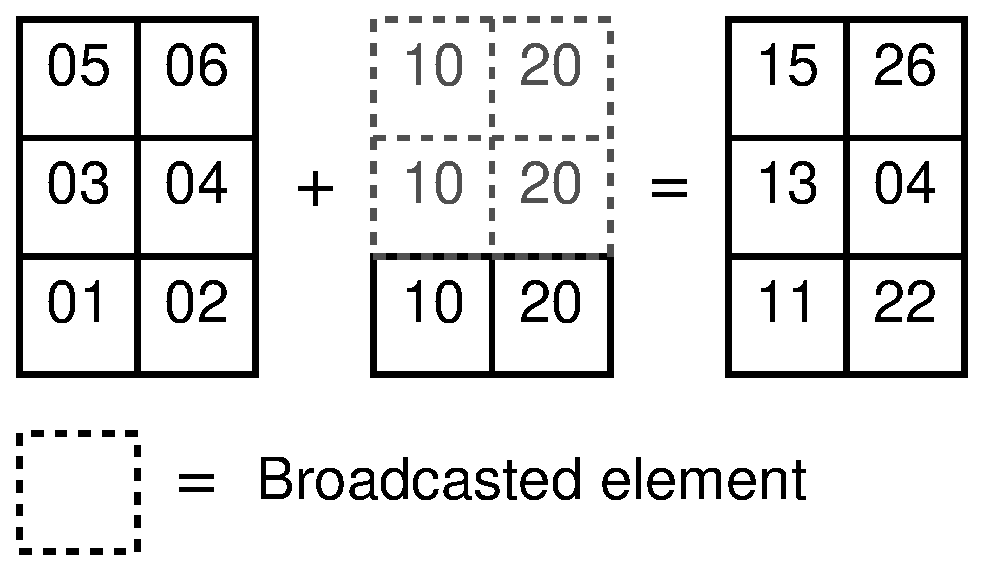
\includegraphics[width=120px]{gfx/ufunc_broadcast}
 \caption{Universal function broadcasting. The ufunc \texttt{addition} is applied on a 3x2 array and a 1x2 array. The first dimension of the 1x2 array is broadcasted to the size of the first dimension of the 3x2 array. The result is a 3x2 array in which the two arrays are added together in an element-by-element fashion.}
 \label{fig:ufunc_broadcast}
\end{figure}


\subsection{Basic Linear Algebra Subprograms}
NumPy makes use of the numerical library Basic Linear Algebra Subprograms (BLAS) \cite{blas79}. A highly optimized BLAS implementation exists for almost all HPC platforms and NumPy exploits this when possible. Operations on vector-vector, matrix-vector and matrix-matrix (BLAS level 1, 2 and 3 respectively) all use BLAS in NumPy. 


\section{DistNumPy}
DistNumPy is a new version of NumPy that parallelizes array operations in a manner completely transparent to the user - from the perspective of the user, the difference between NumPy and DistNumPy is minimal. DistNumPy can use multiple processors through the communication library Message Passing Interface (MPI)\cite{mpi}. However, we have chosen not to follow the standard MPI approach in which the same user-program is executed on all MPI-processes. This is because the standard MPI approach requires the user to differentiate between the MPI-processes, e.g. sequential areas in the user-program must be guarded with a branch based on the MPI-rank of the process. In DistNumPy MPI communication must be fully transparent and the user needs no knowledge of MPI or any parallel programming model. However, the user is required to use the array operations in DistNumPy to obtain any kind of speedup. We think this is a reasonable requirement since it is also required by NumPy.

The only difference in the API of NumPy and DistNumPy is the array creation routines. DistNumPy allow both distributed and non-distributed arrays to co-exist thus the user must specify, as an optional parameter, if the array should be distributed. The following illustrates the only difference between the creation of a standard array and a distributed array:
\lstset{frame=none, xleftmargin=0mm, numbers=none}
\begin{lstlisting}
A = numpy.array([1,2,3])#Non-Distributed
B = numpy.array([1,2,3], dist=True)#Distributed
\end{lstlisting}
\lstset{frame=single, xleftmargin=5mm, numbers=left}


\subsection{Interfaces}
There are two programming interfaces in NumPy - one in Python and one in C. We aim to support the complete Python interface and a great subset of the C interface. However, the part of the C interface that involves direct access to low level data structures will not be supported. It is not feasible to return a C-pointer that represents the elements in a distributed array.


\subsection{Data layout}
Two-Dimensional Block Cyclic Distribution is a very popular distribution scheme and it is used in numerical libraries like ScaLAPACK\cite{Blackford96} and LINPACK\cite{linpack79}. It supports matrices and vectors and has a good load balance in numerical problems that have a diagonal computation workflow e.g. Gaussian elimination. The distribution scheme works by arranging all MPI-processes in a two dimensional grid and then distributing data-blocks in a round-robin fashion either along one or both grid dimensions (Fig. \ref {fig:datalayout}); the result is a well-balanced distribution.

NumPy is not limited to matrices and vectors as it supports arrays with an arbitrary number of dimensions. DistNumPy therefore use a more generalized N-Dimensional Block Cyclic Distribution inspired by High Performance Fortran\cite{Loveman93}, which supports an arbitrary number of dimensions. Instead of using a fixed process grid, we have a process grid for every number of dimensions. This works well when operating on arrays with the same number of dimensions but causes problems otherwise. For instance in a matrix-vector multiplication the two arrays are distributed on different process grid and may therefore require more communication. ScaLAPACK solves the problem by distributing vectors on two-dimensional process grids instead of one-dimensional process grids, but this will result in vector operations that cannot utilize all available processors. An alternative solution is to redistribute the data between a series of identically leveled BLAS operations using a fast runtime redistribution algorithm like \cite{PrylliT97} demonstrates.


\subsection{Operation dispatching}
The MPI-process hierarchy in DistNumPy has one MPI-process (master) placed above the others (slaves). All MPI-processes run the Python interpreter but only the master executes the user-program, the slaves will block at the \texttt{import numpy} statement. 

The following describes the flow of the dispatching:
\begin{enumerate}
\item The master is the dispatcher and will, when the user applies a python command on a distributed array, compose a message with meta-data describing the command. 
\item The message is then broadcasted from the master to the slaves with a blocking MPI-broadcast. It is important to note that the message only contains meta-data and not any actual array data.
\item After the broadcast, all MPI-processes will apply the command on the sub-array they own and exchange array elements as required (Point-to-Point communication).
\item When the command is completed, the slaves will wait for the next command from the master and the master will return to the user's python program. The master will return even though some slaves may still be working on the command, synchronization is therefore required before the next command broadcast.
\end{enumerate}


\begin{figure}
 \centering
 \includegraphics[width=\linewidth]{gfx/datalayout}
 \caption{The Two-Dimensional Block Cyclic Distribution of a matrix on a 2 x 3 grid of processors.}
 \label{fig:datalayout}
\end{figure}


\subsection{Views}
In NumPy an array does not necessarily represent a complete contiguous block of memory. An array is allowed to represent a subpart of another array i.e. it is possible to have a hierarchy of arrays where only one array represent a complete contiguous block of memory and the other arrays represent a subpart of that memory. 

Inspired by NumPy, DistNumPy implements an array hierarchy where distributed arrays are represented by the following two data structures.
\begin{itemize}
\item \textbf{Array-base} is the base of an array and has direct access to the content of the array in main memory. An array-base is created with all related meta-data when the user allocates a new distributed array, but the user will never access the array directly through the array-base. The array-base always describes the whole array and its meta-data such as array size and data type are constant.
\item \textbf{Array-view} is a view of an array-base. The view can represent the whole array-base or only a sub-part of the array-base. An array-view can even represent a non-contiguous sub-part of the array-base. An array-view contains its own meta-data that describe which part of the array-base is visible and it can add non-existing 1-length dimensions to the array-base. The array-view is manipulated directly by the user and from the users perspective the array-view is the array.
\end{itemize}
Array-views are not allowed to refer to each other, which means that the hierarchy is flat with only two levels: array-base below array-view. However, multiple array-views are allowed to refer to the same array-base. This hierarchy is illustrated in Figure \ref{fig:views}. 

\begin{figure}
 \centering
 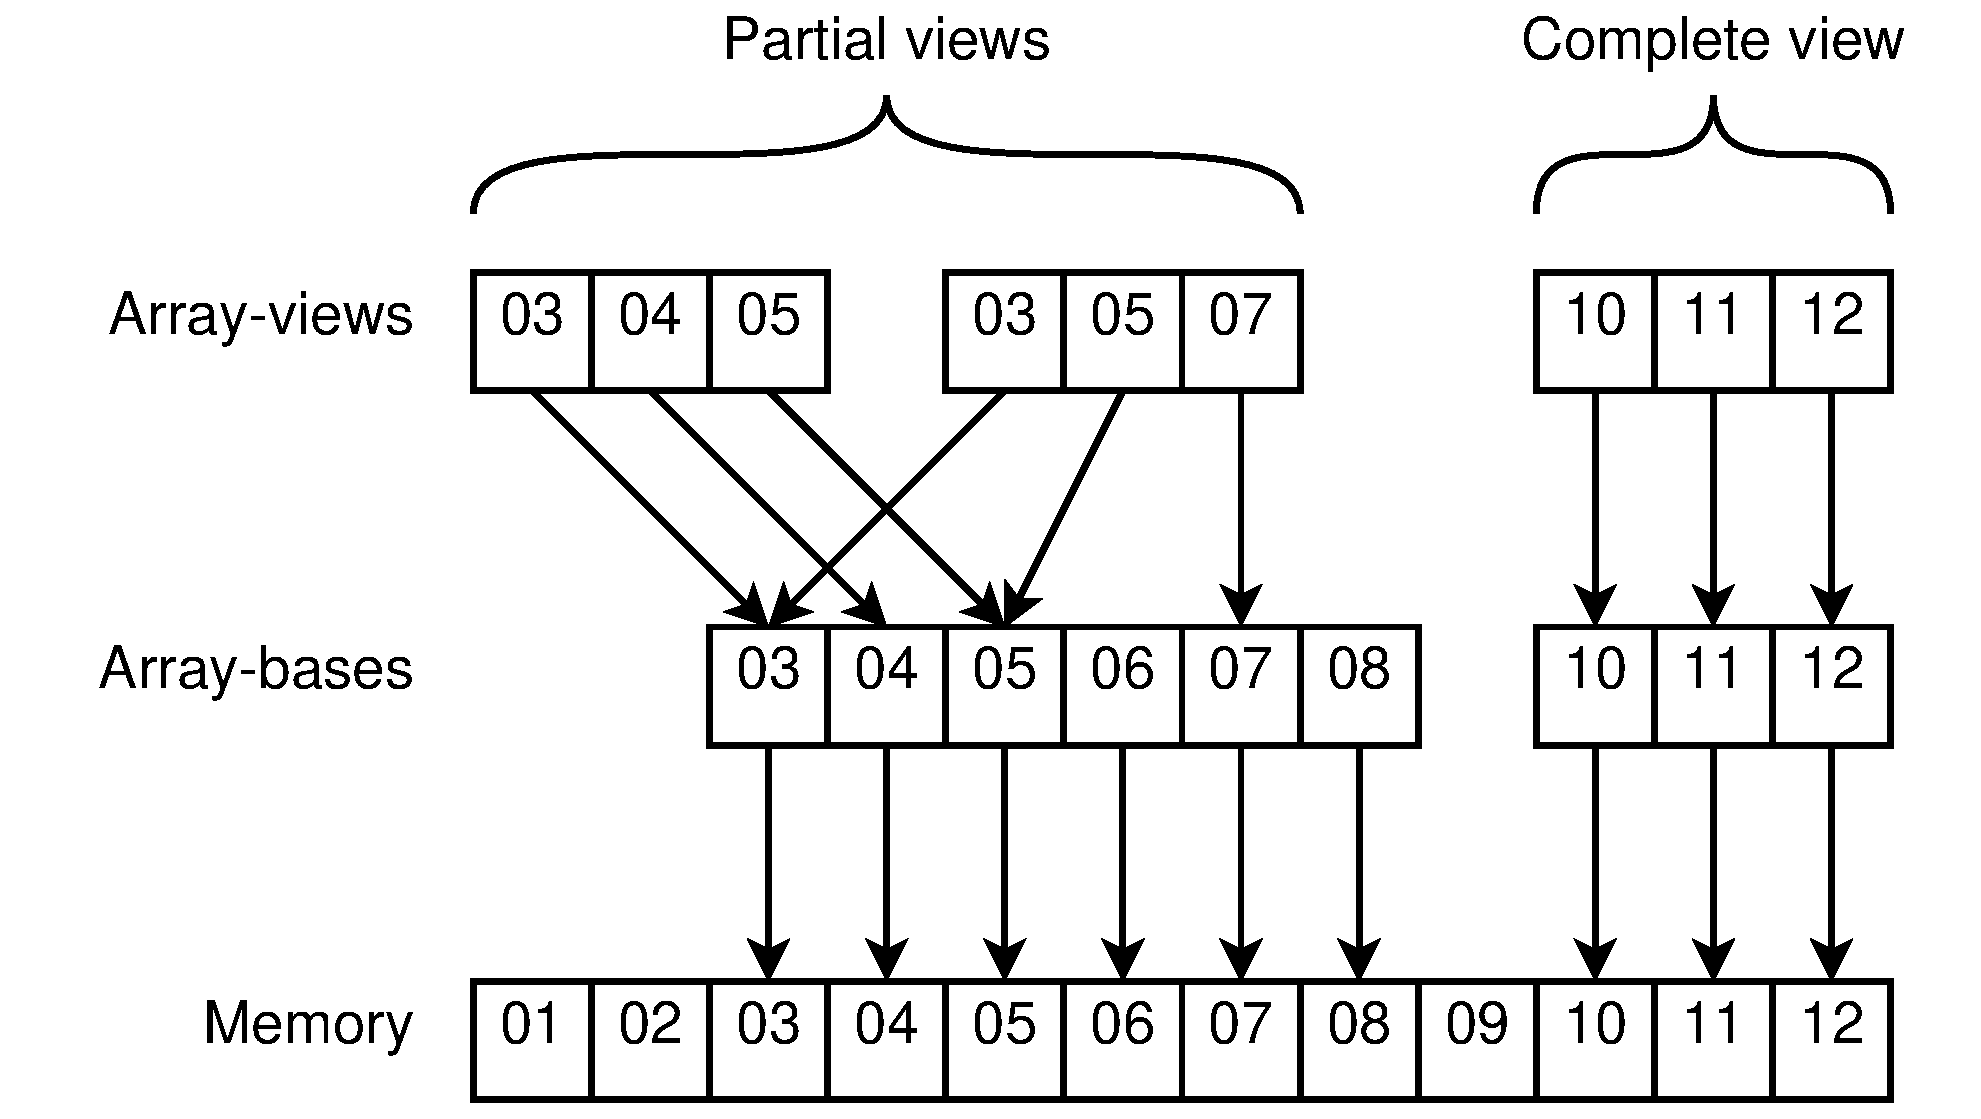
\includegraphics[width=\linewidth]{gfx/views}
 \caption{Reference hierarchy between the two array data structures and the main memory. Only the three array-views at top of the hierarchy are visible from the perspective of the user.}
 \label{fig:views}
\end{figure}

\subsection{Optimization hierarchy}
%We introduce a hierarchy of implementations all optimized for specific operation scenarios because the performance impact when optimizing a NumPy operation in the general case is very limited. It is far easier to optimize and make computational shortcuts if we have some predefined simplifications. When an operation is applied, a search through the hierarchy determines the most optimized implementation for that particular operation. At the bottom of the hierarchy, there is an implementation that can handle all operation scenarios.

%Most simplifications are related to the use of partial views, which are array-views that represents a sub-part of the underlying array-base. It is much simpler to handle array-views that represent the whole array-base 1-to-1 rather than handle arbitrary array-views. For instance, blocking communication together in large MPI-messages becomes difficult and introduces a significant overhead when using non-continuous array-views. The problem is the data distribution scheme (N-Dimensional Block Cyclic Distribution). It becomes hard for an MPI-process to determine which part of its local data the array-view covers. By introducing a simplified scenario that only includes continuous array-views we have implemented a very efficient blocked universal function.

It is a significant performance challenge to support array-views that represent a non-contiguous sub-part of an array-base. The difficulty lies in the process of packing communication and computation together in large blocks, which is very expensive when operating on non-contiguous data. To overcome this problem we introduce a hierarchy of implementations all optimized for specific operation scenarios. When an operation is applied a search through the hierarchy determines the most optimized implementation for that particular operation. All operations have its own hierarchy some with more levels than others, but at the bottom of the hierarchy all operations have an implementation that can handle all scenarios.


\subsection{Parallel BLAS}
As previously mentioned NumPy supports BLAS operations on vectors and matrices. DistNumPy therefore implements a parallel version of BLAS inspired by PBLAS from the ScaLAPACK library. Since DistNumPy uses the same data-layout as ScaLAPACK, it would be straightforward to use PBLAS for all parallel BLAS operations. However, to simplify the installation and maintenance of DistNumPy we have chosen to implement our own parallel version of BLAS. We use SUMMA\cite{SUMMA_GeijnW97} for matrix multiplication, which enable us to use the already available BLAS library locally on the MPI-processes. SUMMA is only applicable on complete array-views and we therefore use a straightforward implementation that computes one element at a time if partial array-views are involved in the computation. 

\subsection{Universal function}
In DistNumPy, the implementation of ufunc uses three different scenarios.
\begin{enumerate}
\item In the simplest scenario we have a perfect match between all elements in the array-views and applying an ufunc does not require any communication between MPI-processes. The scenario is applicable when the ufunc is applied on complete array-views with identical shapes.
\item In the second scenario the array-views must represent a continuous part of the underlying array-base. The computation is parallelized by the data distribution of the output array and data blocks from the input arrays are fetched when needed. We use non-blocking one-side communication (\texttt{MPI\_Get}) when fetching data blocks, which makes it possible to compute one block while fetching the next block (double buffering).
\item The final scenario does not use any simplifications and works with any kind of array-view. It also uses non-blocking one-side communication but only one element at a time.
\end{enumerate}


\section{Examples}\label{sec:examples}
To evaluate DistNumPy we have implemented three Python programs that all make use of NumPy's vector-operations (ufunc). They are all optimized for a sequential execution on a single CPU and the only program change we make, when going from the original NumPy to our DistNumPy, is the array creation argument \texttt{dist}. 
A walkthrough of a Monte Carlo simulation is presented as an example of how DistNumPy handles Python executions.


\subsection{Monte Carlo simulation}
\begin{figure}
\begin{lstlisting}
from numpy import *
(x, y) = (empty([S], dist=True), \
          empty([S], dist=True))
(x, y) = (random(x), random(y))
(x, y) = (square(x), square(y))
z = (x + y) < 1
print add.reduce(z) * 4.0 / S #The result
\end{lstlisting}
 \caption{Computing Pi using Monte Carlo simulation. \texttt{S} is the number of samples used. We have defined a new ufunc (\texttt{ufunc\_random}) to make sure that we use an identical random number generator in all benchmarks. The ufunc uses "\texttt{rand()/(double)RAND\_MAX}" from the ANSI C standard library (\texttt{stdlib.h}) to generate numbers.}
 \label{lst:montecarlo}
\end{figure}

We have implemented an efficient Monte Carlo Pi simulation using NumPy's ufunc. The implementation is a translation of the Monte Carlo simulation included in the benchmark suite SciMark 2.0\cite{SciMark}, which is written in Java. It is very simple and uses two vectors with length equal the number of samples used in the calculation. Because of the memory requirements, this drastically reduces the maximum number of samples. Combining multiple simulations will allow more samples but we will only use one simulation. The implementation is included in its full length (Fig. \ref{lst:montecarlo}) and the following is a walkthrough of a simulation (the bullet-numbers represents line numbers):

\begin{enumerate}
\item[\textbf{1:}] All MPI-processes interpret the \texttt{import} statement and initiate DistNumPy. Besides calling \texttt{MPI\_Init()} the initialization is identical to the original NumPy but instead of returning from the import statement, the slaves, MPI-processes with rank greater than zero, listen for a command message from the master, the MPI-process with rank zero.
\item[\textbf{2-3:}] The master sends two \texttt{CREATE\_ARRAY} messages to all slaves. The two messages contain an array shape and unique identifier (UID), which in this case identifies \texttt{x} and \texttt{y}, respectively. All MPI-processes allocate memory for the arrays and stores the array information.
\item[\textbf{4:}] The master sends two \texttt{UFUNC} messages to all slaves. Each message contains a UID and a function name \texttt{ufunc\_random}. All MPI-processes apply the function on the array with the specified UID. A pointer to the function is found by calling \texttt{PyObject\_Get} \texttt{AttrString} with the function name. It is thereby possible to support all ufuncs from NumPy.
\item[\textbf{5:}] Again the master sends two \texttt{UFUNC} messages to all slaves but this time with function name \texttt{square}.
\item[\textbf{6:}] The master sends a \texttt{UFUNC} messages with function name \texttt{add} followed by a \texttt{UFUNC} messages with function name \texttt{less\_than}. The scalar \texttt{1} is also in the message.
\item[\textbf{7:}] The master sends a \texttt{UFUNC\_REDUCE} messages with function name \texttt{add}. The result is a scalar, which is not distributed, and the master therefore solely computes the remainder of the computation and print the result. When the master is done a \texttt{SHUTDOWN} message is sent to the slaves and the slaves call \texttt{exit(0)}.
\end{enumerate}


\subsection{Jacobi method}
\begin{figure}
\begin{lstlisting}
h = zeros(shape(B), float, dist=True)
dmax = 1.0
AD = A.diagonal()
while(dmax > tol):
  hnew = h + (B - add.reduce(A * h, 1)) / AD
  tmp = absolute((h - hnew) / h)
  dmax = maximum.reduce(tmp)
  h = hnew
print h #The result
\end{lstlisting}
 \caption{Iteratively Jacobi solver for matrix \texttt{A} with solution vector \texttt{B} both are distributed arrays. The \texttt{import} statement and the creation of \texttt{A} and \texttt{B} is not included here.
 \texttt{tol} is the maximum tolerated value of the diagonal-element with the highest value (\texttt{dmax}).}
 \label{lst:jocobi}
\end{figure}

The Jacobi method is an algorithm for determining the solutions of a system of linear equations. It is an iterative method that uses a spitting scheme to approximate the result.

Our implementation uses ufunc operations in a while-loop until it converges. Most of the implementation is included here(Fig. \ref{lst:jocobi}).


\subsection{Newtonian N-body simulation}
A Newtonian N-body simulation is one that studies how bodies, represented by a mass, a location, and a velocity, move in space according to the laws of Newtonian physics. We use a straightforward algorithm computing all body-body interactions. The NumPy implementation is a direct translation of a MATLAB program\cite{assignmentNbody}. The working loop of the two implementations take up 19 lines in Python and 22 lines in MATLAB thus it is too big to include here. However, the implementation is straightforward and use universal functions and matrix multiplications.


\section{Experiments}
In this section, we will conduct performance benchmarks on DistNumPy and NumPy\footnote{NumPy version 1.3.0}. We will benchmark the three Python programs presented in Section \ref{sec:examples}. All benchmarks are executed on two different Linux clusters -- an Intel Core 2 Quad cluster and an Intel Nehalem cluster. Both clusters consist of processors with four CPU-cores, but the number of processors per node differs. Intel Core 2 Quad cluster has one CPU per node whereas the Intel Nehalem cluster has two CPUs per node. The interconnect is Gigabit Ethernet in both clusters. (Table \ref{tab:specs}).

Our experiments consist of a speedup benchmark, which we define as an execution time comparison between a sequential execution with NumPy and a parallelized execution with DistNumPy while the input is identical. Strong-scaling is used in all benchmarks and the input size is therefore constant.

%To investigate the performance difference between using a single CPU-core and multiple CPU-cores per node, we include speedup graphs that show the two scenarios. 

%We define a strong-scale benchmark as a comparison between a sequential execution with NumPy and a parallelized execution with DistNumPy where the input size is fixed. We define a weak-scale benchmark similar but with an input that scales linearly with the number of CPU-cores.

\begin{table}
\caption{Hardware specifications}
\centering
\begin{tabular}{|lll|}
\hline
CPU & Core 2 Quad & Nehalem\\
CPU Frequency & 2.26 GHz & 2.66 GHz\\
CPU per node & 1 & 2\\
Cores per CPU & 4 & 4\\
Memory per node & 8 GB @ 6.5 GB/s & 24 GB @ 25.6 GB/s\\
Number of nodes & 8 & 8\\
Network & Gigabit Ethernet & Gigabit Ethernet\\
\hline
\end{tabular}

\label{tab:specs}
\end{table}
%Core 2 Quad: http://ark.intel.com/Product.aspx?id=35365
%Nehalem: http://ark.intel.com/Product.aspx?id=40200


\subsection{Monte Carlo simulation}
A Distributed Monte Carlo simulation is embarrassingly parallel and requires a minimum of communication.  This is also the case when using DistNumPy because ufuncs are only applied on identically shaped arrays and it is therefore the simplest ufunc scenario. Additionally, the implementation is CPU-intensive because a complex ufunc is used as random number generator. 

The result of the speedup benchmark is illustrated in Figure \ref{fig:MonteCarlo}. We see a close to linear speedup for the Nehalem cluster - a CPU utilization of 88\% is achieved on 64 CPU-cores. The penalty of using multiple CPU-cores per node is noticeable on the Core 2 architecture - a CPU utilization of 68\% is achieved on 32 CPU-cores.

\begin{figure*}[t]%
  \begin{center}%
    \subfloat[\label{fig:MonteCarloStrong}]{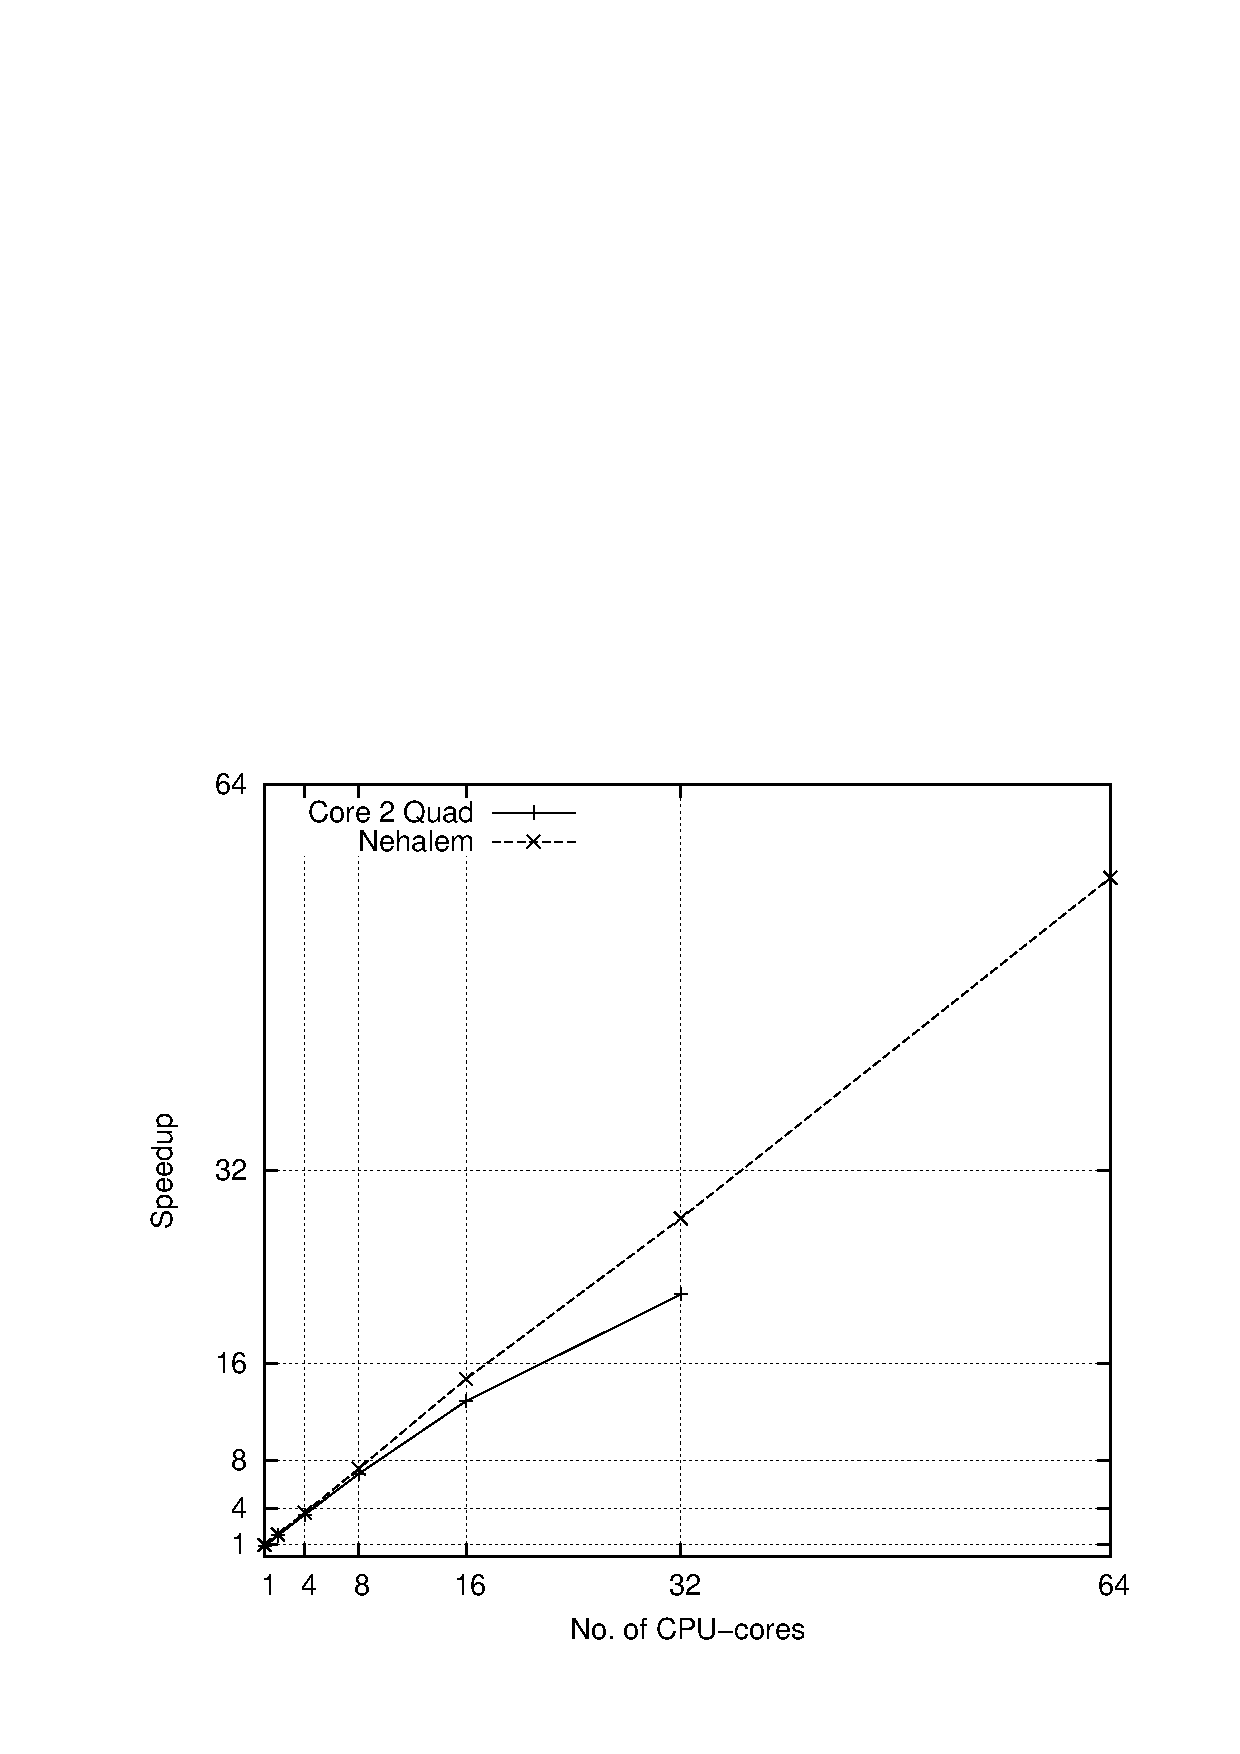
\includegraphics[width=230px]{gfx/MonteCarloStrong}}
%    \qquad
    \subfloat[\label{fig:MonteCarloStrongSMP}]{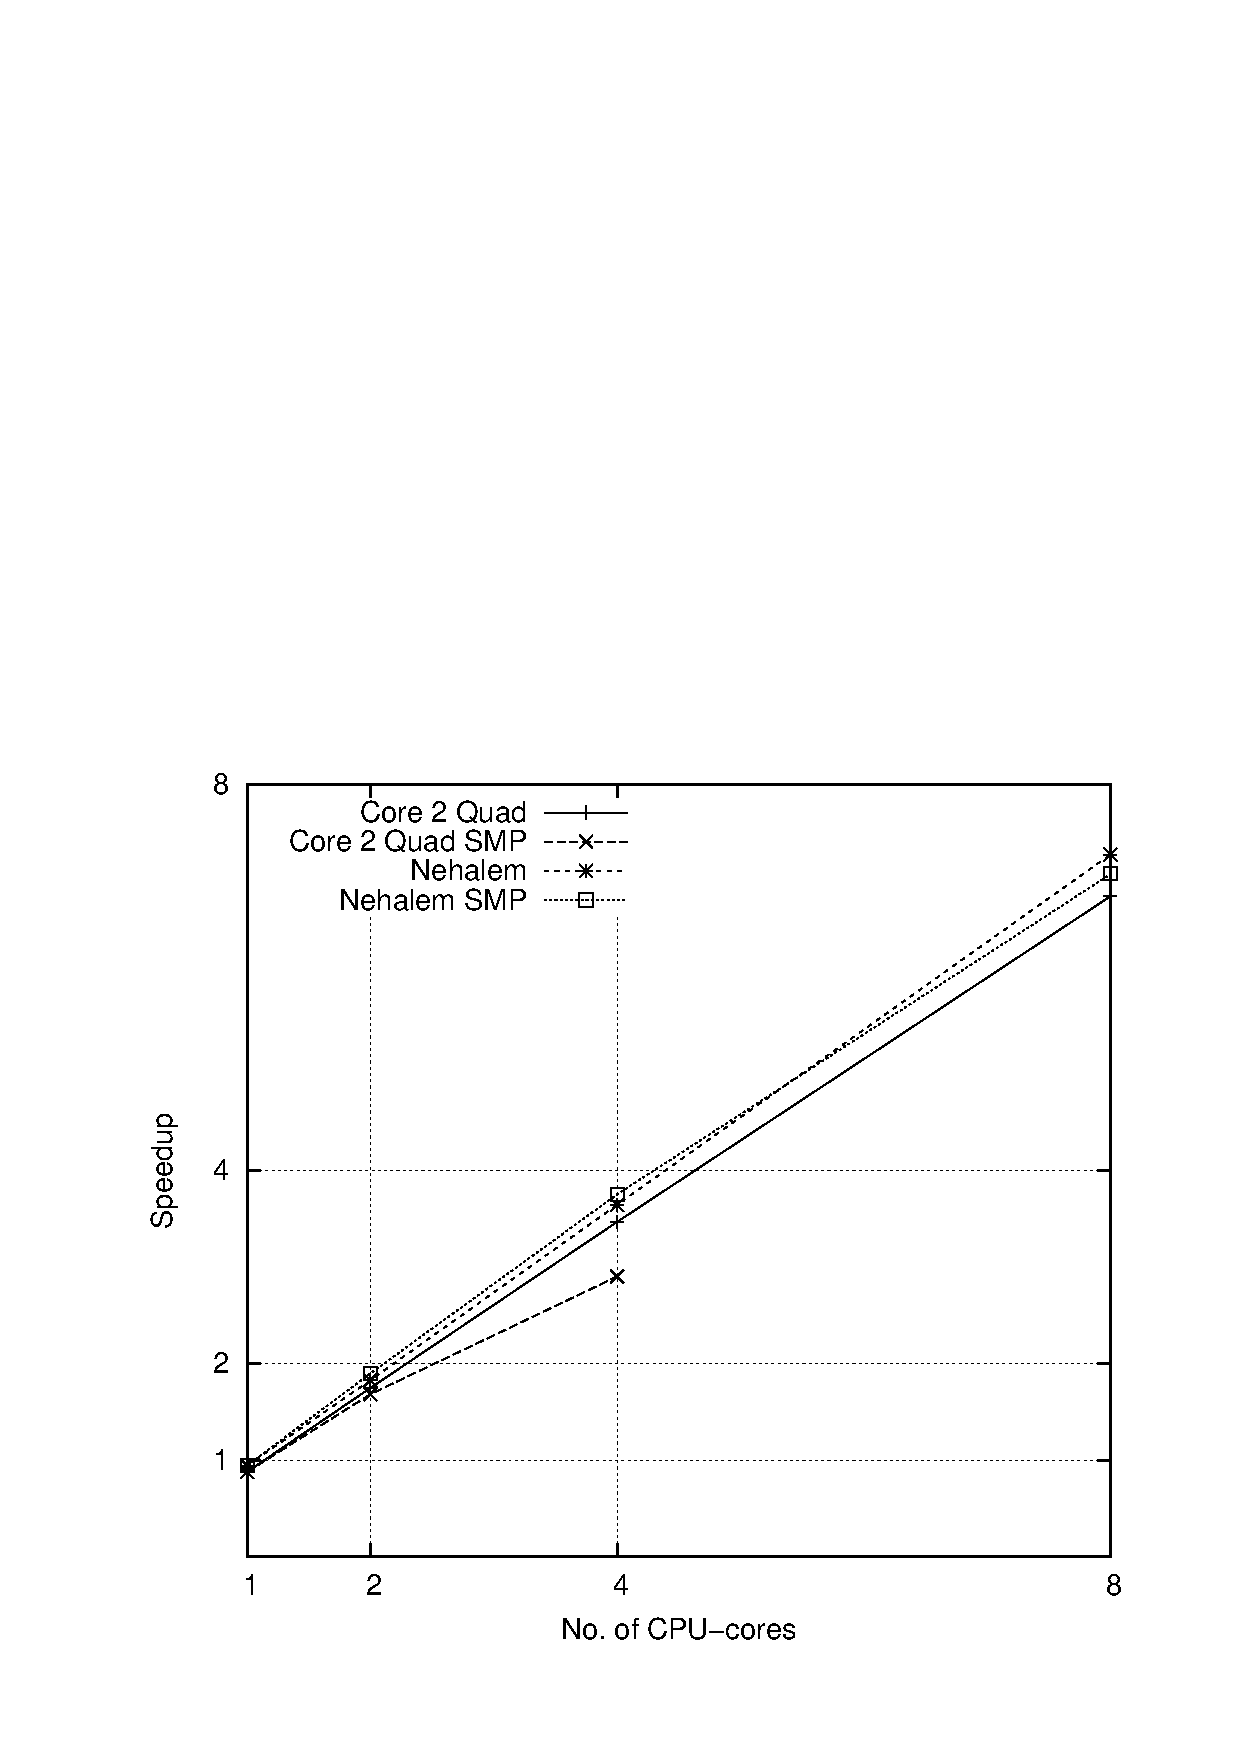
\includegraphics[width=230px]{gfx/MonteCarloStrongSMP}}
    \caption{Speedup of the Monte Carlo simulation. In graph (a) the two architectures uses a minimum number of CPU-cores per node. Added in graph (b) is the result of using multiple CPU-cores on a single node (SMP).}%
    \label{fig:MonteCarlo}%
  \end{center}
\end{figure*}


\subsection{Jacobi method}
The dominating part of the Jacobi method, performance-wise, is the element-by-element multiplication of \texttt{A} and \texttt{h} (Fig. \ref{lst:jocobi} line 5). It consists of $O(n^2)$ operations where as all the other operations only consist $O(n)$ operations. Since scalar-multiplication is a very simple operation, the dominating ufunc in the implementation is memory-intensive.

The result of the speedup benchmark is illustrated in Figure \ref{fig:JacobiScale}. We see a good speedup with 8 CPU-cores and to some degree also with 16 Nehalem CPU-cores. However, the CPU utilization when using more than 16 CPU-cores is very poor. The problem is memory bandwidth - since we use multiple CPU-cores per node when using more than 8 CPU-cores, the aggregated memory bandwidth of the Core 2 cluster does only increase up to 8 CPU-cores. The Nehalem cluster is a bit better because it has two memory buses per node, but using more than 16 CPU-cores will not increase the aggregated memory bandwidth.


\subsubsection{Profiling of the Jacobi implementation}
%To get a better picture of the memory bandwidth limitation observed in the Jacobi execution we have profiled the execution (Fig. \ref{fig:JacobiProfiling}). The percentages used with communication increases as expected when the number of CPU-cores increases. However, the profile different between eight CPU-cores and sixteen CPU-cores is minimal, which is due to the limited memory bandwidth. Since each cluster-node makes use of multiple CPU-cores when more than eight CPU-cores are used the memory bandwidth limitation increases the communication time drastically. 

To get a better picture of the execution efficiency the Jacobi execution is profiled by measuring the time used on computation and on communication (Fig. \ref{fig:JacobiProfiling}). As expected the percentages used with communication increases as the number of CPU-cores increases. 


%\begin{figure}
% \centering
% 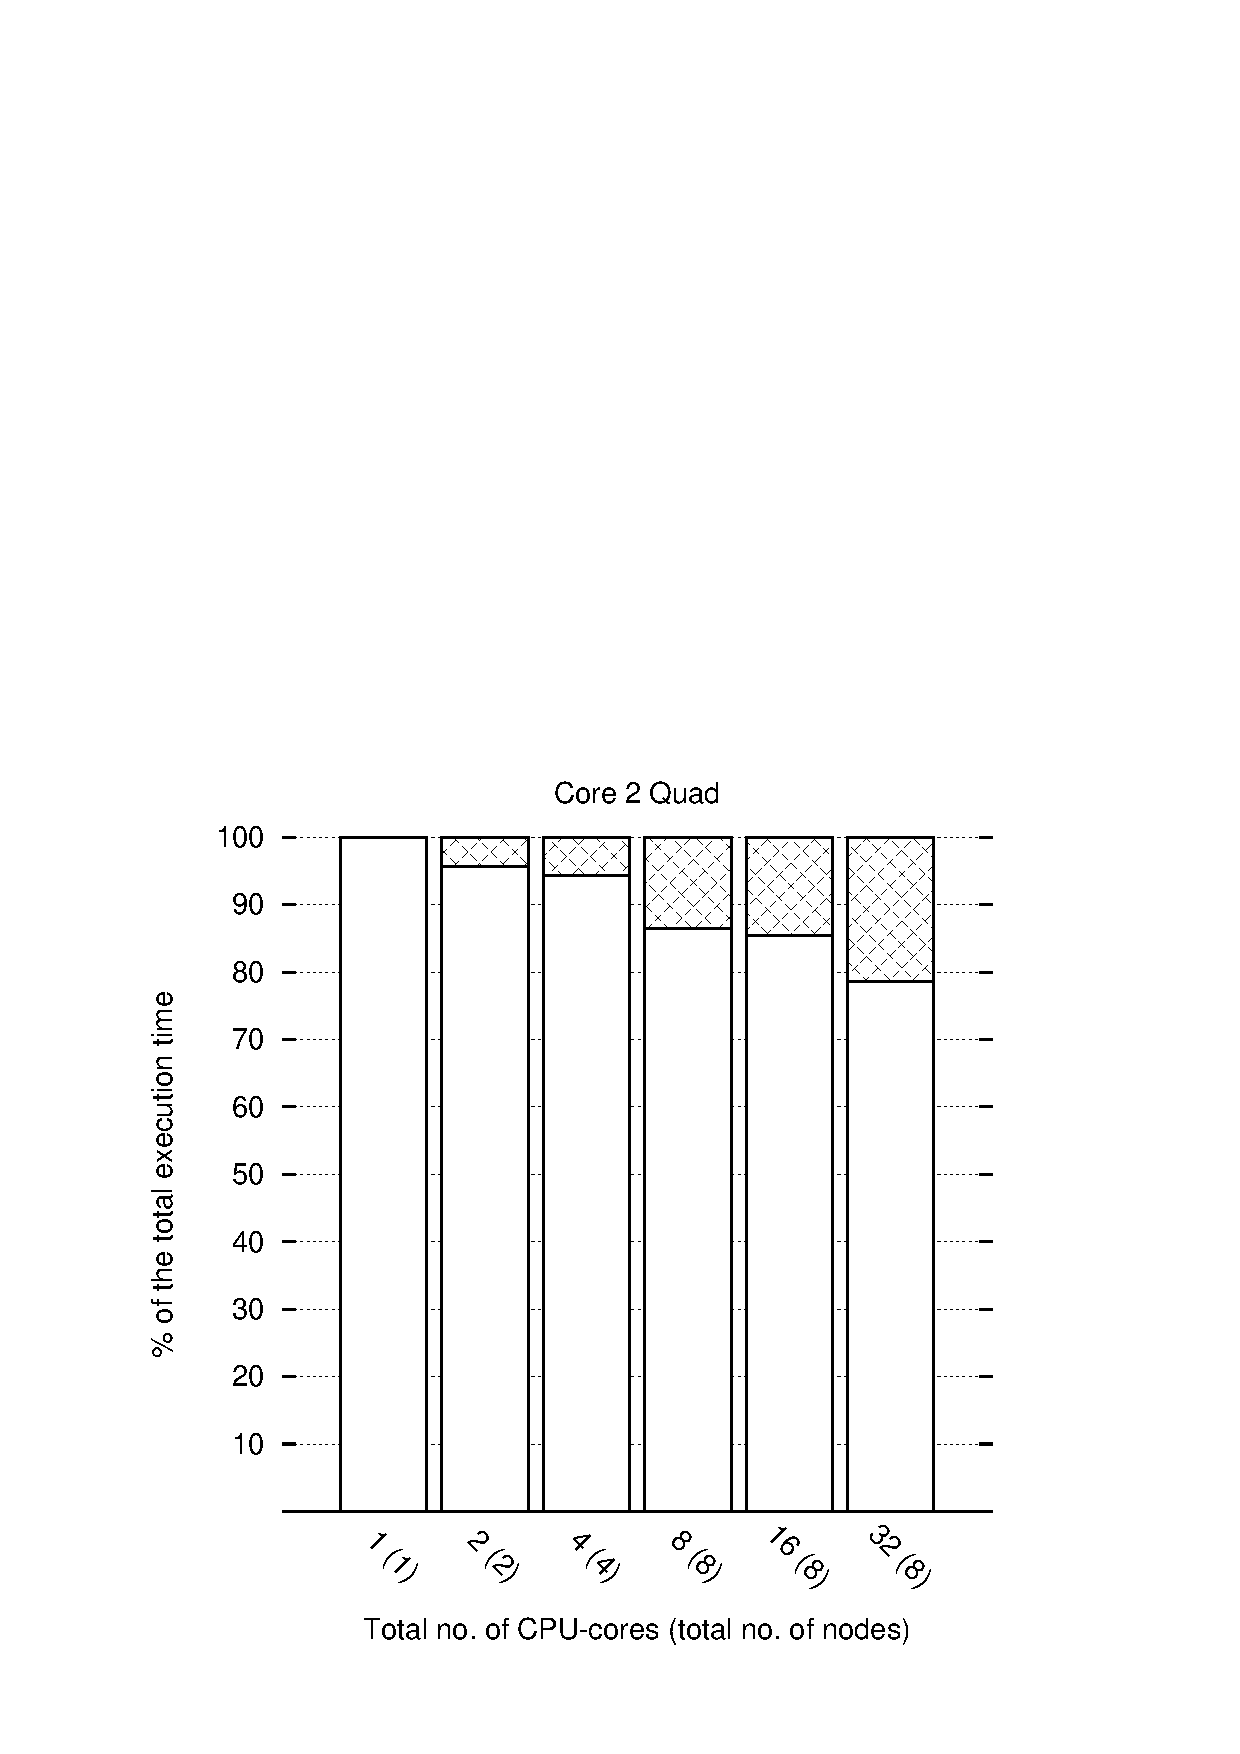
\includegraphics[width=230px]{gfx/JacobiProfiling}
% \caption{Profiling of the Jacobi implementation. The figure illustrate the relationship between communication and computation in percentages. }
% \label{fig:JacobiProfiling}
%\end{figure}

\begin{figure*}[t]%
  \begin{center}%
    \subfloat[\label{fig:JacobiStrong}]{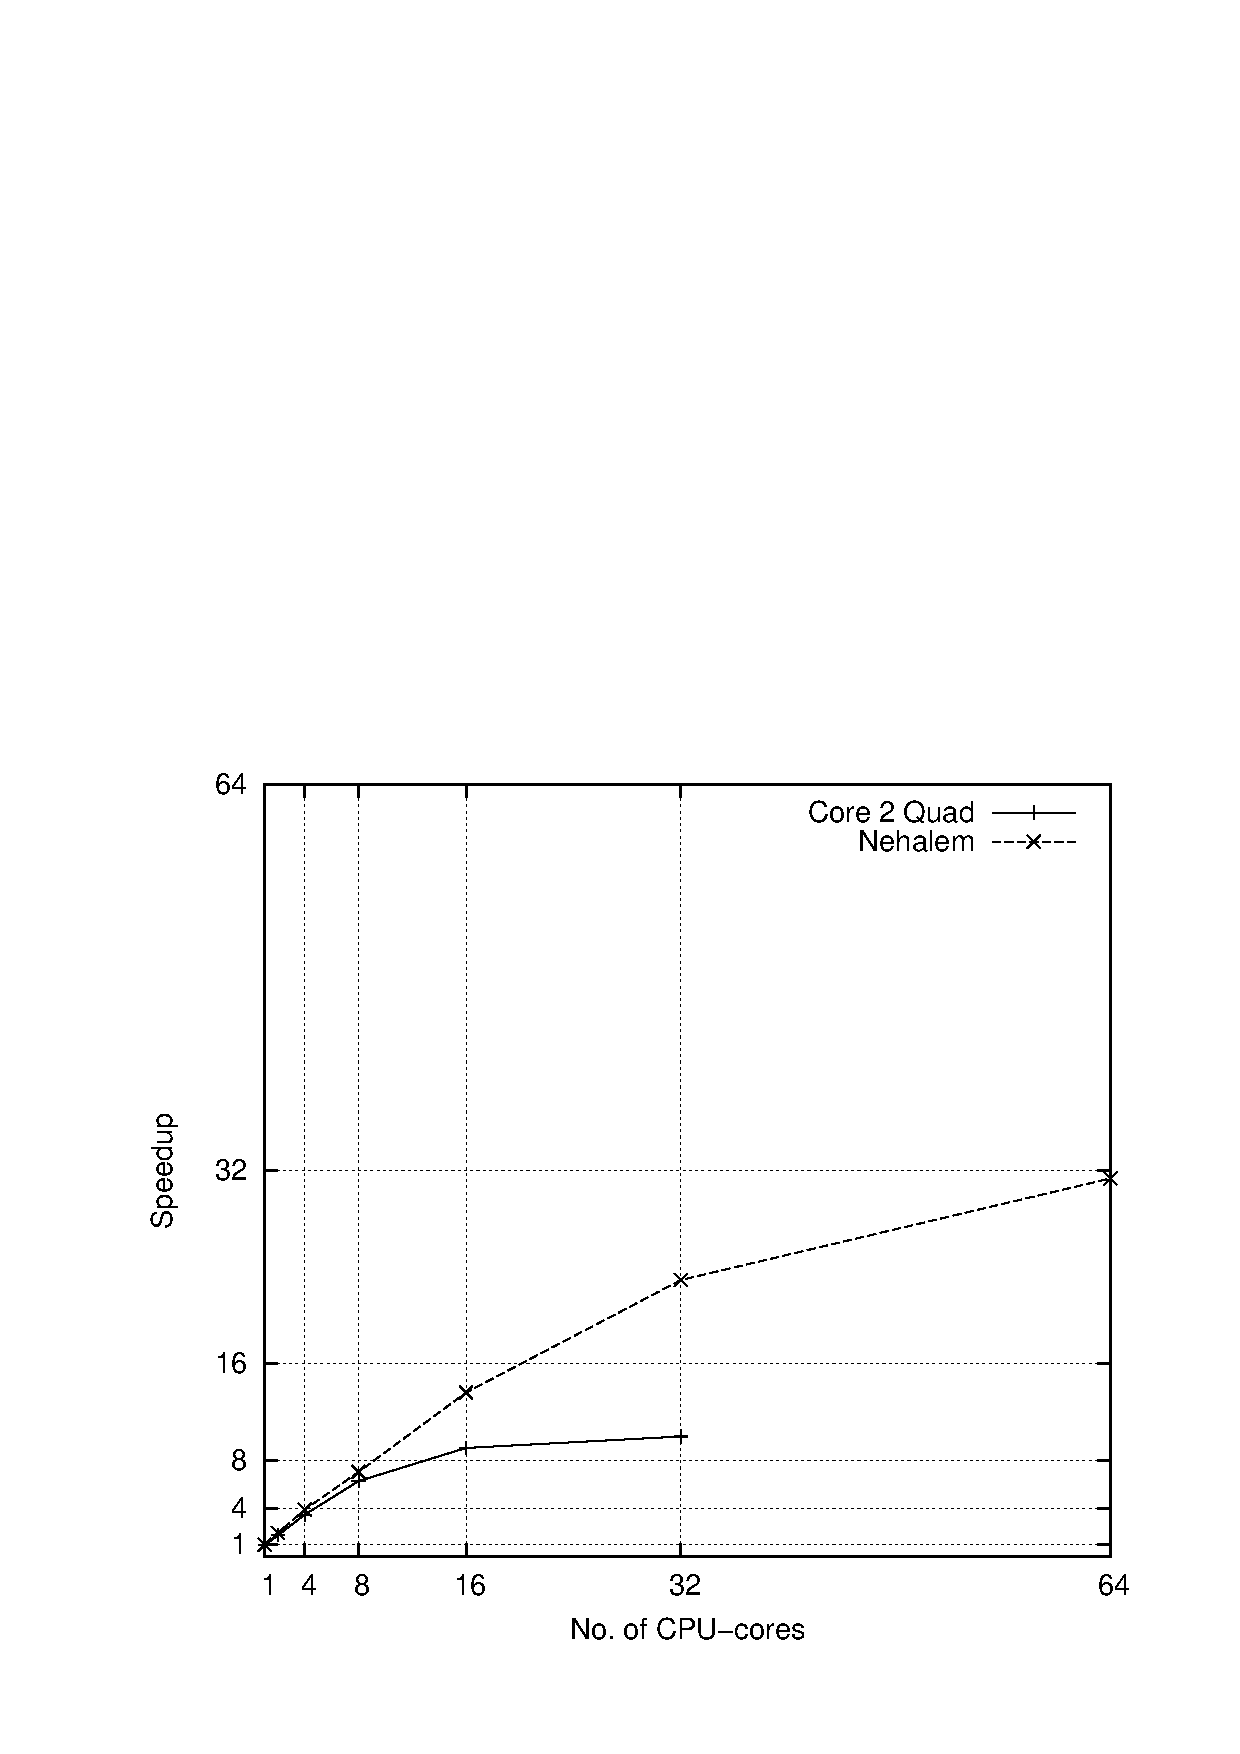
\includegraphics[width=230px]{gfx/JacobiStrong}}
%    \qquad
    \subfloat[\label{fig:JacobiStrongSMP}]{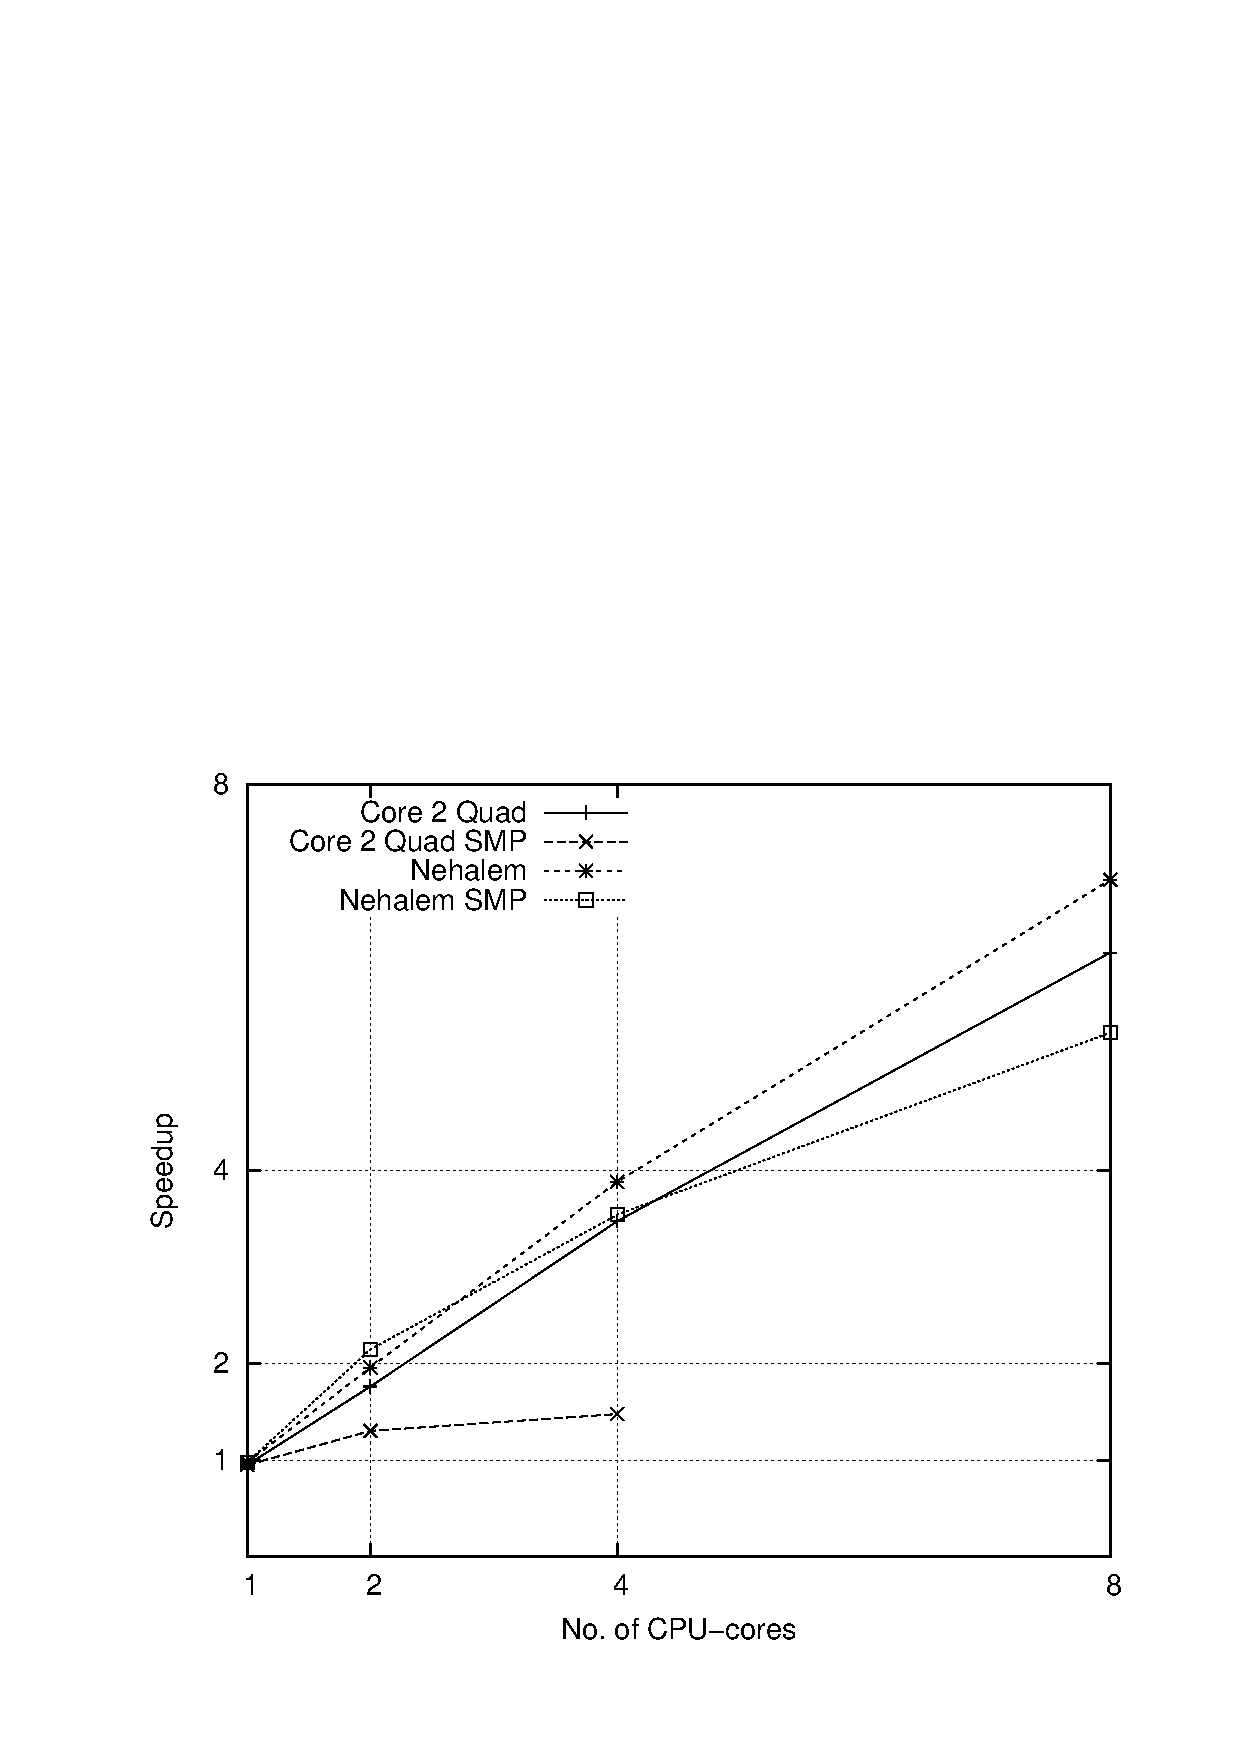
\includegraphics[width=230px]{gfx/JacobiStrongSMP}}
    \caption{Speedup of the Jacobi solver. In graph (a) the two architectures uses a minimum number of CPU-cores per node. Added in graph (b) is the result of using multiple CPU-cores on a single node (SMP).}%
    \label{fig:JacobiScale}%
  \end{center}
\end{figure*}

\begin{figure*}[t]%
  \begin{center}%
    \subfloat[\label{fig:JacobiProfiling1}]{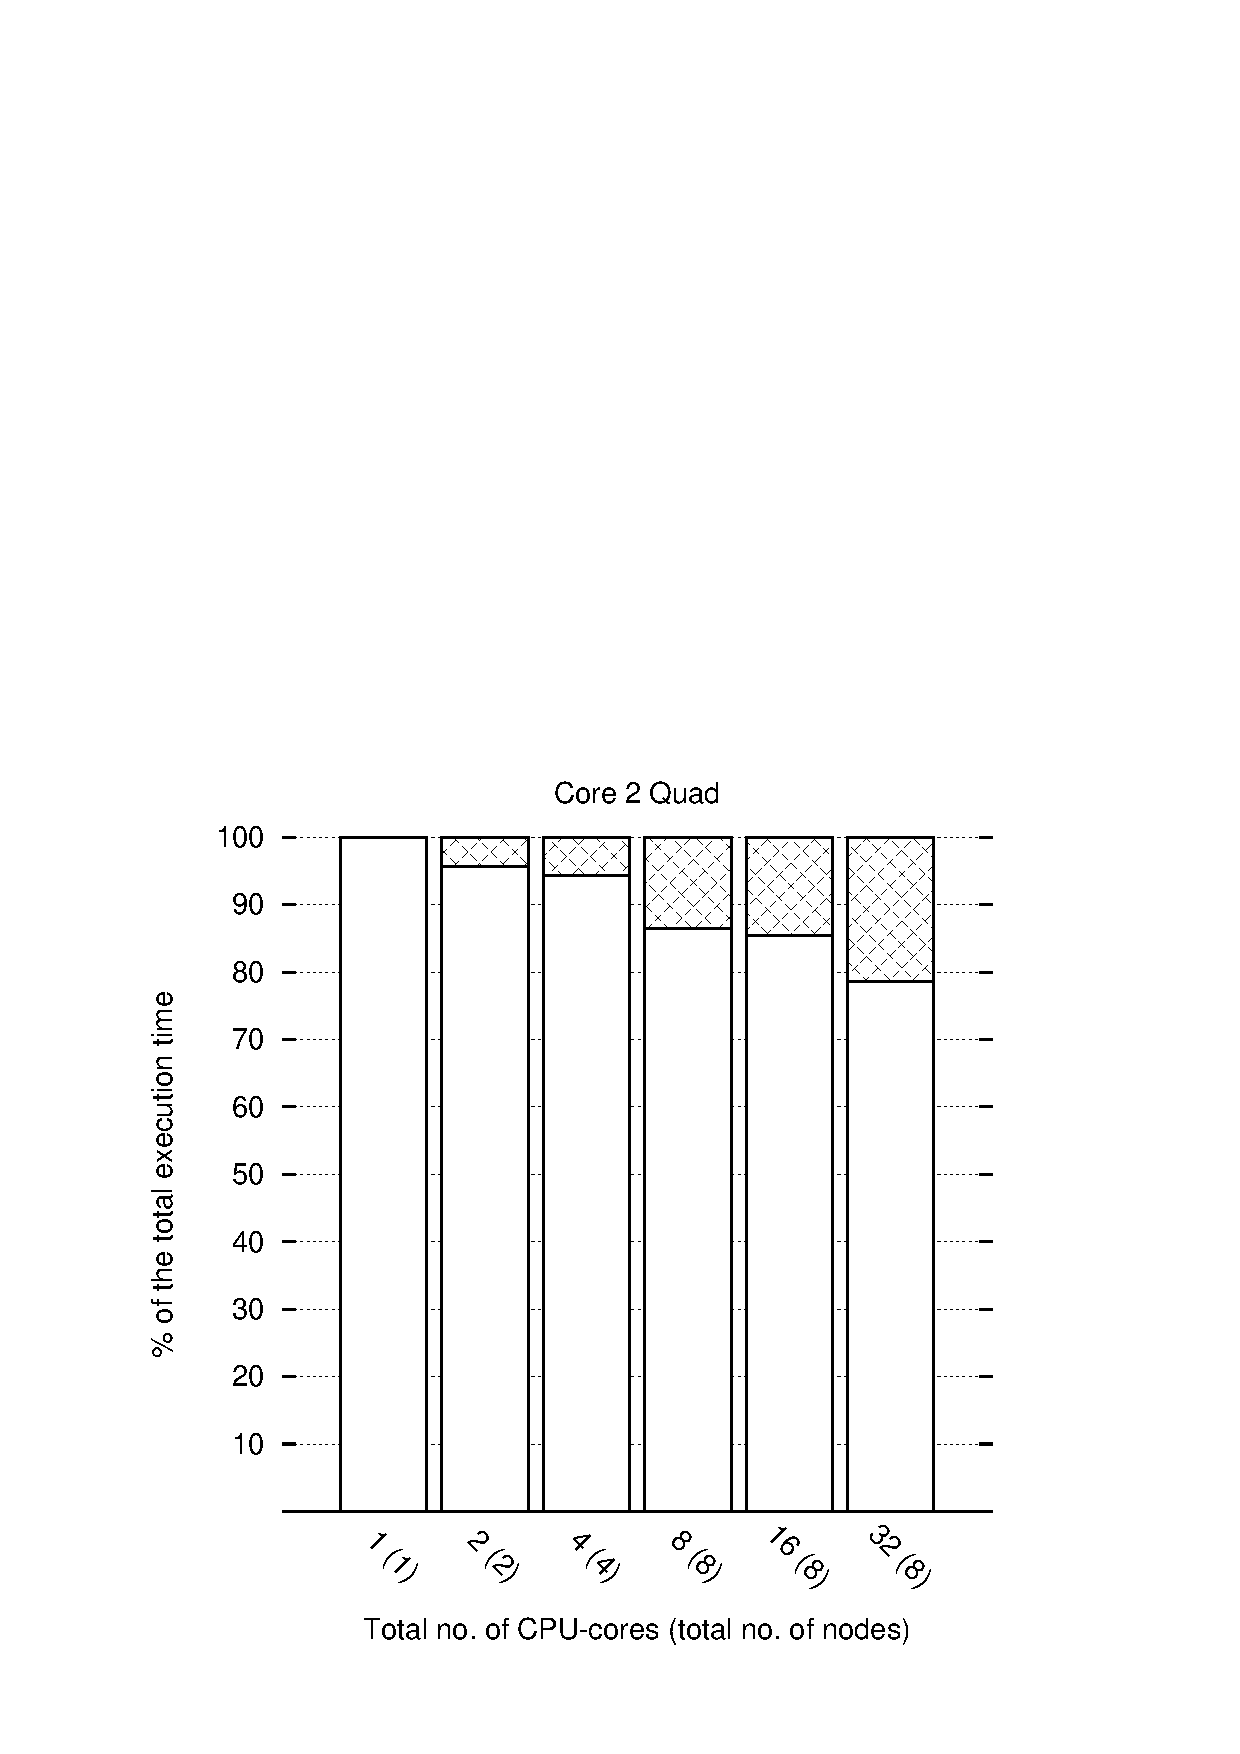
\includegraphics[width=255px]{gfx/JacobiProfiling}}
%    \qquad
    \subfloat[\label{fig:JacobiProfiling2}]{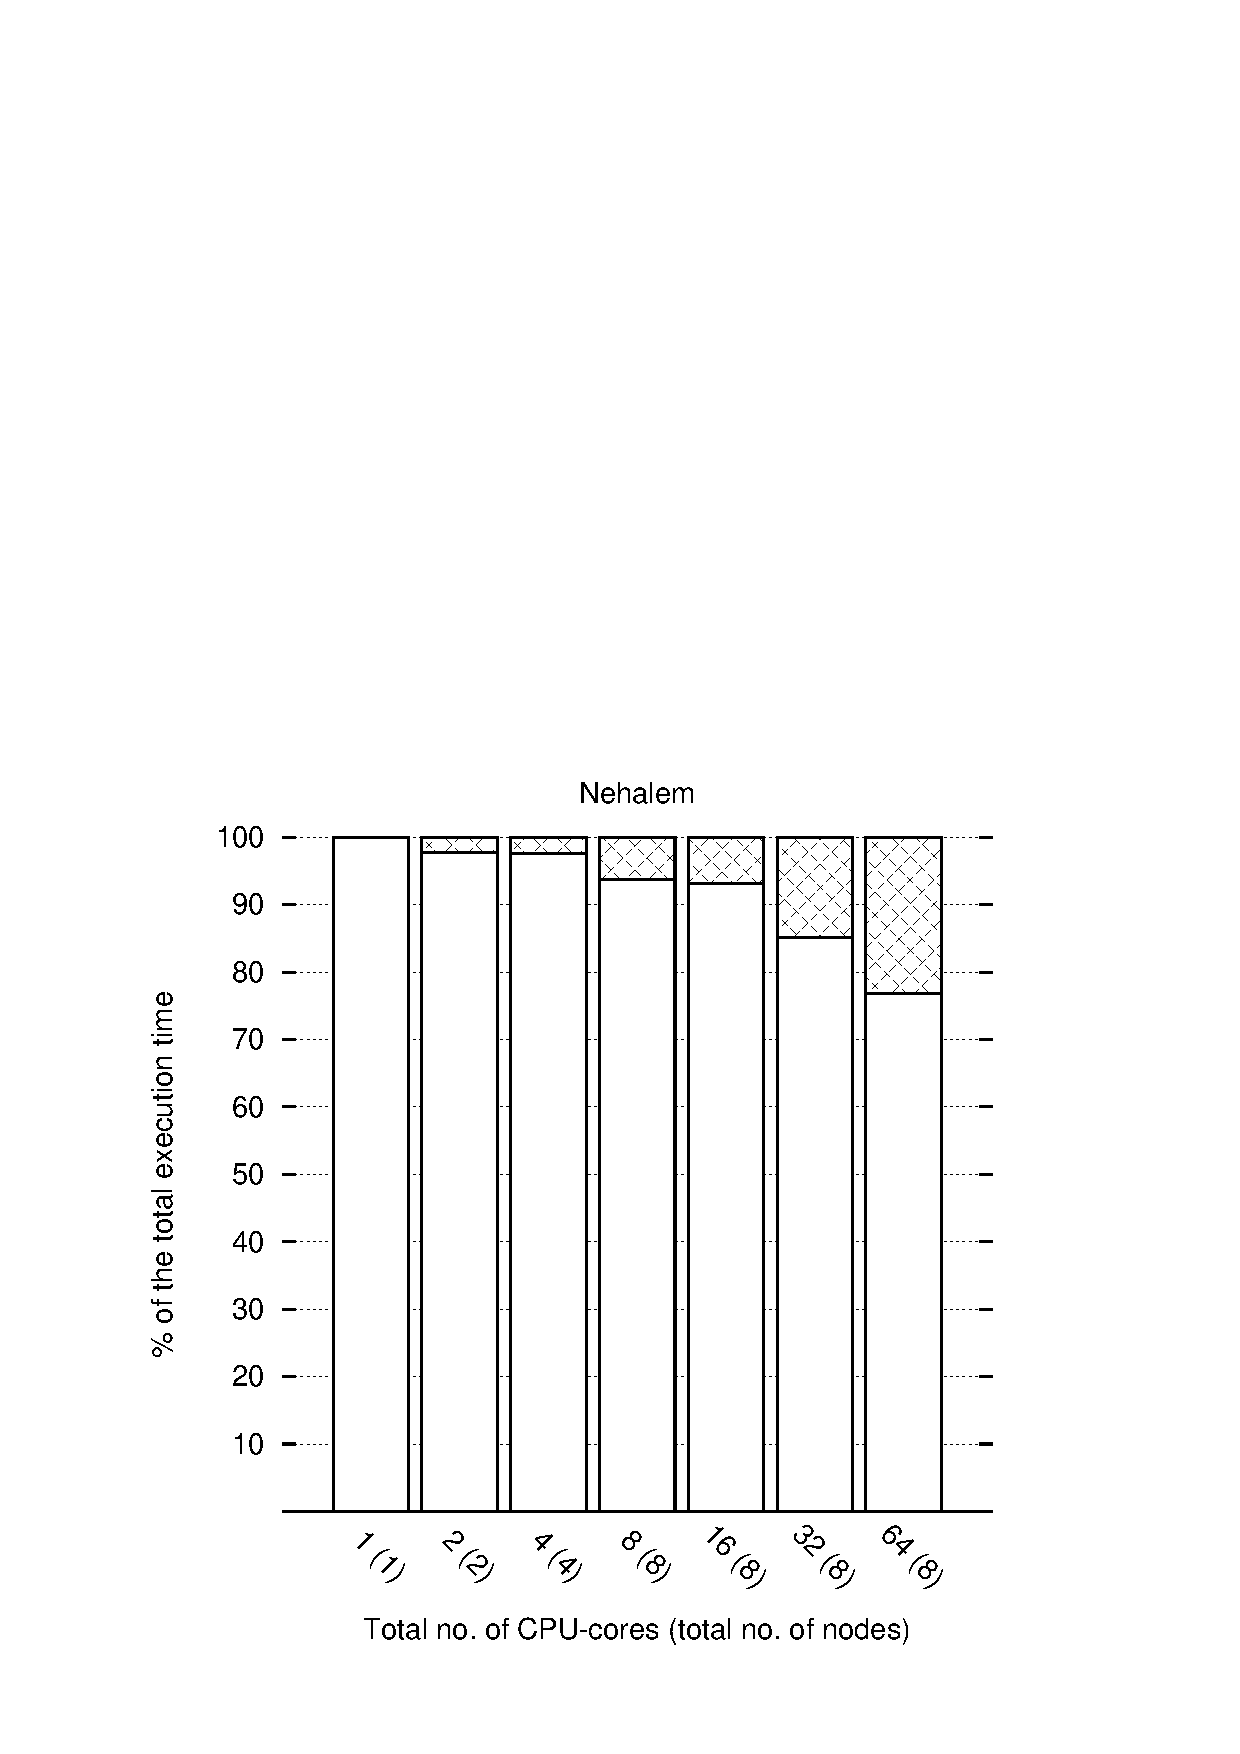
\includegraphics[width=255px]{gfx/JacobiProfiling2}}
    \caption{Profiling of the Jacobi experiment. The two figures illustrate the relationship between communication and computation when running on the Core 2 Quad architecture (a) and the Nehalem architecture (b), respectively. The area with the check pattern represent MPI communication and the clean area represent computation. Note that these figures relates directly to the Jacobi speedup graph (Fig \ref{fig:JacobiStrong}).}
    \label{fig:JacobiProfiling}%
  \end{center}
\end{figure*}


\subsection{Newtonian N-body simulation}
The result of the speedup benchmark is illustrated in Figure \ref{fig:NbodyScale}. Compared to the Jacobi method we see a similar speedup and CPU utilization. This is expected because the dominating operations are also simple ufuncs. Even though there are some matrix-multiplications, which have a great scalability, it is not enough to significantly boost the overall scalability.

\begin{figure*}%
  \begin{center}%
    \subfloat[\label{fig:NbodyStrong}]{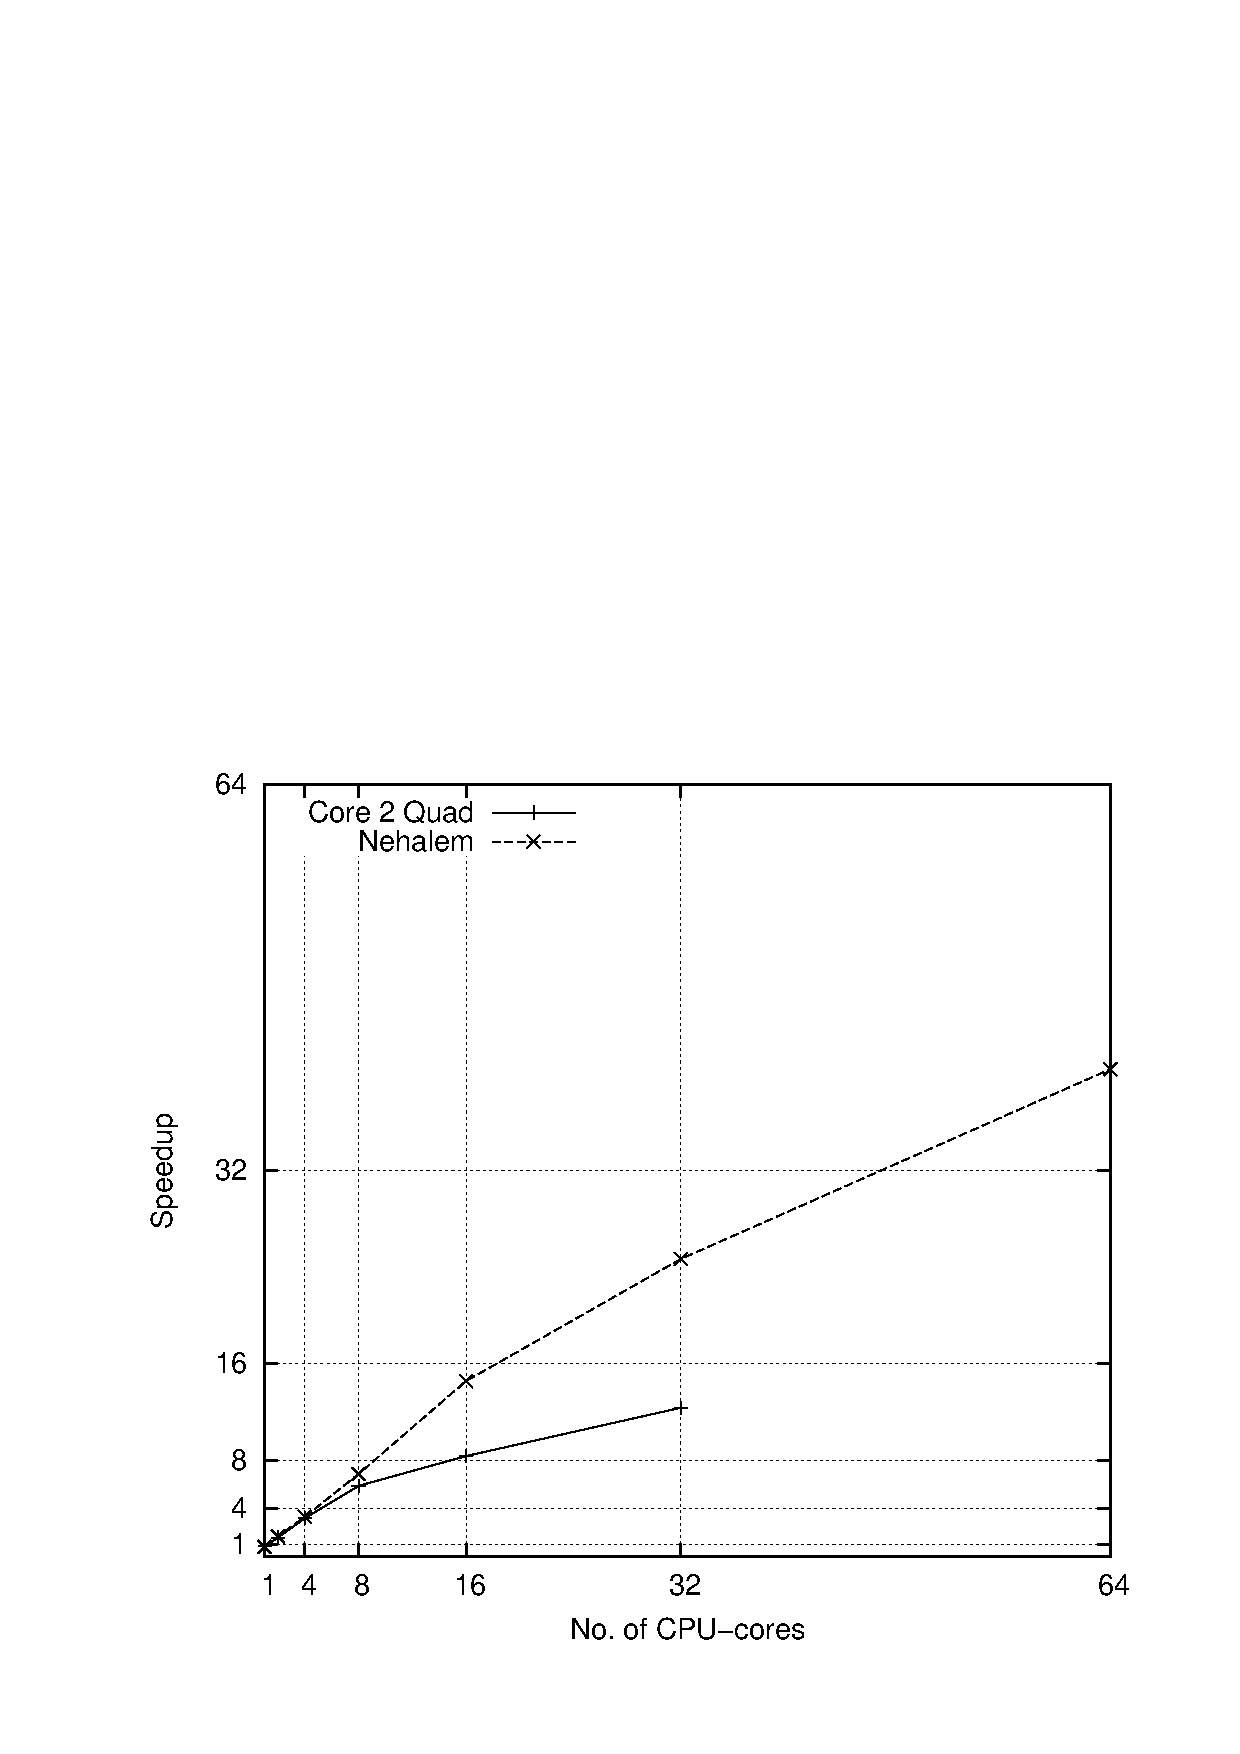
\includegraphics[width=230px]{gfx/NbodyStrong}}
%    \qquad
    \subfloat[\label{fig:NbodyStrongSMP}]{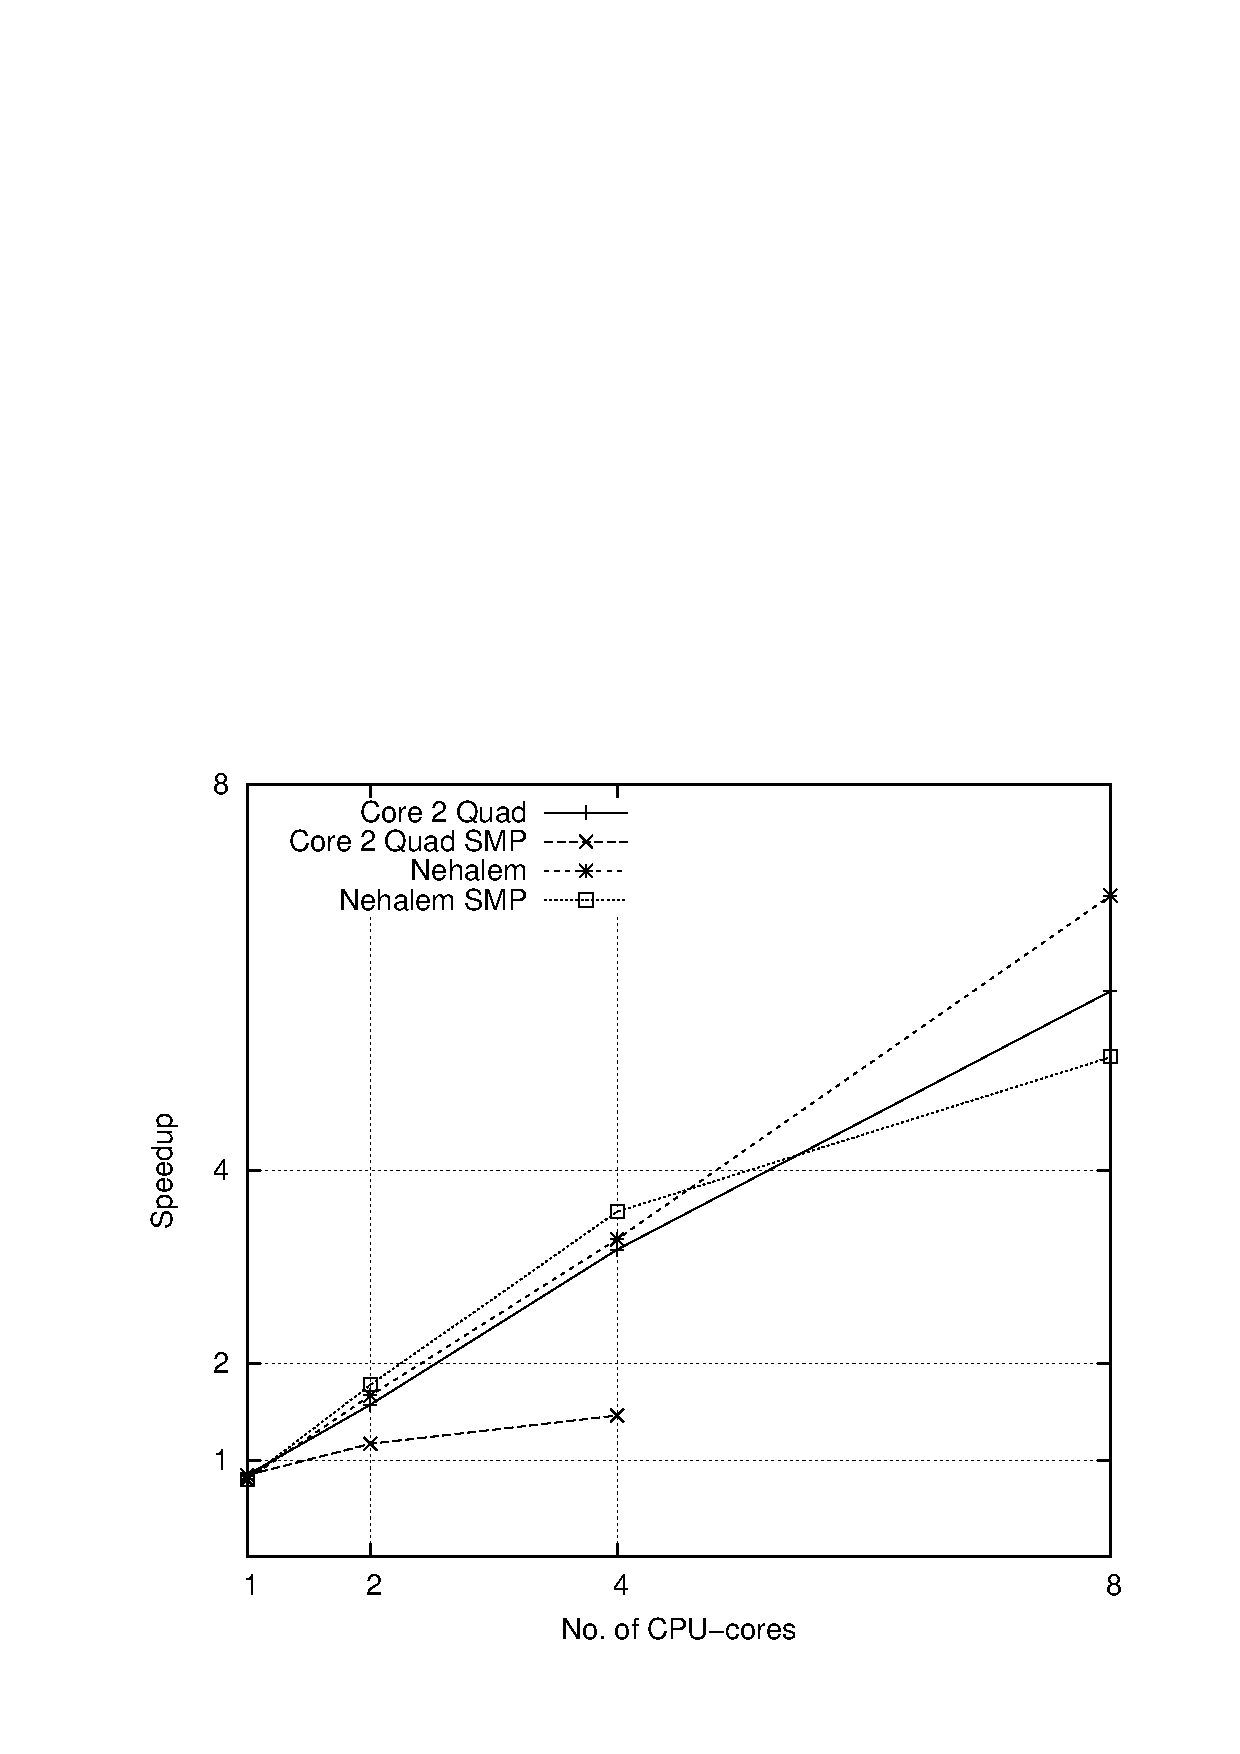
\includegraphics[width=230px]{gfx/NbodyStrongSMP}}
    \caption{Speedup of Newtonian N-body simulation. In graph (a) the two architectures uses a minimum number of CPU-cores per node. Added in graph (b) is the result of using multiple CPU-cores on a single node (SMP).}%
    \label{fig:NbodyScale}%
  \end{center}
\end{figure*}


\subsection{Alternative programming language}
DistNumPy introduces a performance overhead compared to a lower-level programming language such as C/C++ or Fortran. To investigate this overhead we have implemented the Jacobi benchmark in C. The implementation uses the same sequential algorithm as the NumPy and DistNumPy implementations. 

Executions on both architectures show that DistNumPy and NumPy is roughly 50\% slower than the C implementation when executing the Jacobi method on one CPU-core. This is in rough runtime numbers: 21 seconds for C, 31 seconds for NumPy and 32 seconds for DistNumPy.

Obviously highly hand-optimized implementations have a clear performance advantages over DistNumPy. For instance by the use of a highly optimized implementation in C \cite{Kristensen09} demonstrates extreme scalability of a similar Jacobi computation -- an execution by 16384 CPU-cores achieves a CPU utilization of 70\% on a Blue Gene/P architecture. 

\subsection{Summary}
The benchmarks clearly show that DistNumPy has both good performance and scalability when execution is not bound by the memory bandwidth, which is evident from looking at the CPU utilization when only one CPU-core per node is used. As expected the scalability of the Monte Carlo simulation is better than the Jacobi and the N-body computation because of the reduced communication requirements and more CPU-intensive ufunc operation. 

The scalability of the Jacobi and the N-body computation is drastically reduced when using multiple CPU-cores per node. The problem is the complexity of the ufunc operations. As opposed to the Monte Carlo simulation, which makes use of a complex ufunc, the Jacobi and the N-body computation only use simple ufuncs e.g. add and multiplication.

As expected the performance of the C implementation is better than the DistNumPy implementation. However, by utilizing two CPU-cores it is possible to outperform the C implementation in the case of the Jacobi method. This is not a possibility in the case of the Monte Carlo simulation where the algorithm does not favor vectorization.

\section{Future work}
In its current state DistNumPy does not implement the NumPy interface completely. Many specialized operations like Fast Fourier transform or LU factorization is not implemented, but it is our intention to implement the complete Python interface and most of the C interface.

Other important future work include performance and scalability improvement. As showed by the benchmarks, applications that are dominated by non-complex ufuncs easily become memory bounded. One solutions is to block ufuncs, that operate on common arrays, together in one joint operation and thereby make the joint operation more CPU-intensive. If it is possible to join enough ufuncs together the application may become CPU bound rather than memory bound.

\section{Conclusions}
In this work we have successfully shown that it is possible to implement a parallelized version of NumPy\cite{numpy} that seamlessly utilize distributed memory architectures. The only API difference between NumPy and our parallelized version, DistNumPy, is an extra optional parameter in the array creation routines.

Performance measurements of three Python program, which make use of DistNumPy, show very good performance and scalability. A CPU utilization of 88\% is achieved on a 64 CPU-core Nehalem cluster running a CPU-intensive Monte Carlo simulation. A more memory-intensive N-body simulation achieves a CPU utilization of 91\% on 16 CPU-cores but only 63\% on 64 CPU-cores. Similar a Jacobi solver achieves a CPU utilization of 85\% on 16 CPU-cores and 50\% on 64 CPU-cores.

To obtain good performance with NumPy the user is required to make use of array operations rather than using Python loops. DistNumPy take advantage of this fact and parallelizes array operations. Thus most efficient NumPy applications should be able to benefit from DistNumPy with the distribution parameter as the only change.

We conclude that it is possible to obtain significant speedup with DistNumPy. However, further work is needed if shared memory machines are to be fully utilized as nodes in a scalable architecture.

%\acks

%Acknowledgments, if needed.

% We recommend abbrvnat bibliography style.

\bibliographystyle{abbrvnat}

% The bibliography should be embedded for final submission.

\begin{thebibliography}{18}
\providecommand{\natexlab}[1]{#1}
\providecommand{\url}[1]{\texttt{#1}}
\expandafter\ifx\csname urlstyle\endcsname\relax
  \providecommand{\doi}[1]{doi: #1}\else
  \providecommand{\doi}{doi: \begingroup \urlstyle{rm}\Url}\fi

\bibitem[Anderson et~al.(1990)Anderson, Bai, Dongarra, Greenbaum, McKenney,
  Du~Croz, Hammerling, Demmel, Bischof, and Sorensen]{lapack90}
E.~Anderson, Z.~Bai, J.~Dongarra, A.~Greenbaum, A.~McKenney, J.~Du~Croz,
  S.~Hammerling, J.~Demmel, C.~Bischof, and D.~Sorensen.
\newblock Lapack: a portable linear algebra library for high-performance
  computers.
\newblock In \emph{Supercomputing {'}90: Proceedings of the 1990 ACM/IEEE
  conference on Supercomputing}, pages 2--11, Los Alamitos, CA, USA, 1990. IEEE
  Computer Society Press.
\newblock ISBN 0-89791-412-0.

\bibitem[Blackford(1996)]{Blackford96}
L.~S. Blackford.
\newblock Scalapack.
\newblock In \emph{Proceedings of the 1996 ACM/IEEE conference on
  Supercomputing (CDROM) - Supercomputing 96 Supercomputing 96}, page~5, 1996.
\newblock \doi{10.1145/369028.369038}.

\bibitem[Carlson et~al.(1999)Carlson, Draper, Culler, Yelick, Brooks, and
  Warren]{Carlson99_UPC}
W.~W. Carlson, J.~M. Draper, D.~Culler, K.~Yelick, E.~Brooks, and K.~Warren.
\newblock Introduction to upc and language specification.
\newblock Technical Report CCS-TR-99-157, Bowie, MD, May 1999.

\bibitem[Casanova(2008)]{assignmentNbody}
H.~Casanova.
\newblock N-body simulation assignment, Nov 2008.
\newblock URL
  \url{http://navet.ics.hawaii.edu/~casanova/courses/ics632_fall08/projects.html}.

\bibitem[Dongarra et~al.(1979)Dongarra, Bunch, Moler, and Stewart]{linpack79}
J.~Dongarra, J.~Bunch, C.~Moler, and G.~Stewart.
\newblock Linpack users' guide.
\newblock \emph{SIAM}, 1, 1979.

\bibitem[Geijn and Watts(1997)]{SUMMA_GeijnW97}
R.~A. v.~d. Geijn and J.~Watts.
\newblock Summa: scalable universal matrix multiplication algorithm.
\newblock \emph{Concurrency - Practice and Experience}, 9\penalty0
  (4):\penalty0 255--274, 1997.

\bibitem[Gropp et~al.(1994)Gropp, Lusk, and Skjellum]{mpi}
W.~Gropp, E.~Lusk, and A.~Skjellum.
\newblock \emph{Using MPI Portable Parallel Programming with the Message
  Passing Interface}.
\newblock The MIT Press, 1994.

\bibitem[Guide(1998)]{guide1998mathworks}
M.~U. Guide.
\newblock The mathworks.
\newblock \emph{Inc., Natick, MA}, 5, 1998.

\bibitem[Hill et~al.(2008)Hill, Hambley, Forster, Mewissen, Sloan, Scharinger,
  Trew, and Ghazal]{Hill08}
J.~Hill, M.~Hambley, T.~Forster, M.~Mewissen, T.~M. Sloan, F.~Scharinger,
  A.~Trew, and P.~Ghazal.
\newblock Sprint: a new parallel framework for r.
\newblock \emph{BMC Bioinformatics}, 9:\penalty0 558, 2008.
\newblock \doi{10.1186/1471-2105-9-558}.

\bibitem[Kristensen et~al.(2009)Kristensen, Happe, and Vinter]{Kristensen09}
M.~R.~B. Kristensen, H.~H. Happe, and B.~Vinter.
\newblock Gpaw optimized for blue gene/p using hybrid programming.
\newblock \emph{Parallel and Distributed Processing Symposium, International},
  2009.
\newblock \doi{10.1109/IPDPS.2009.5160936}.

\bibitem[Lawson et~al.(1979)Lawson, Hanson, Kincaid, and Krogh]{blas79}
C.~L. Lawson, R.~J. Hanson, D.~R. Kincaid, and F.~T. Krogh.
\newblock Basic linear algebra subprograms for fortran usage.
\newblock \emph{ACM Trans. Math. Softw.}, 5\penalty0 (3):\penalty0 308--323,
  1979.
\newblock \doi{10.1145/355841.355847}.

\bibitem[Loveman(1993)]{Loveman93}
D.~Loveman.
\newblock High performance fortran.
\newblock \emph{IEEE Parallel \& Distributed Technology: Systems \&
  Applications}, 1\penalty0 (1):\penalty0 25, 1993.
\newblock \doi{10.1109/88.219857}.

\bibitem[Nieplocha et~al.(1996)Nieplocha, Harrison, and
  Littlefield]{Nieplocha96}
J.~Nieplocha, R.~J. Harrison, and R.~J. Littlefield.
\newblock Global arrays: A nonuniform memory access programming model for
  high-performance computers.
\newblock \emph{The Journal of Supercomputing}, 10\penalty0 (2), 1996.
\newblock \doi{10.1007/BF00130708}.

\bibitem[Numrich and Reid(1998)]{Co-arrayFortran98}
R.~W. Numrich and J.~Reid.
\newblock Co-array fortran for parallel programming.
\newblock \emph{SIGPLAN Fortran Forum}, 17\penalty0 (2):\penalty0 1--31, 1998.
\newblock ISSN 1061-7264.
\newblock \doi{10.1145/289918.289920}.

\bibitem[Oliphant(2007)]{numpy}
T.~E. Oliphant.
\newblock Python for scientific computing.
\newblock \emph{Computing in Science and Engineering}, 9:\penalty0 10--20,
  2007.
\newblock ISSN 1521-9615.
\newblock \doi{10.1109/MCSE.2007.58}.

\bibitem[P{\'{e}}rez and Granger(2007)]{PER-GRA:2007}
F.~P{\'{e}}rez and B.~E. Granger.
\newblock Ipython: a system for interactive scientific computing.
\newblock \emph{Comput. Sci. Eng.}, 9\penalty0 (3):\penalty0 21--29, may 2007.
\newblock URL \url{http://ipython.scipy.org}.

\bibitem[Pozo and Miller(2002)]{SciMark}
R.~Pozo and B.~Miller.
\newblock Scimark 2.0, 12 2002.
\newblock URL \url{http://math.nist.gov/scimark2/}.

\bibitem[Prylli and Tourancheau(1997)]{PrylliT97}
L.~Prylli and B.~Tourancheau.
\newblock Fast runtime block cyclic data redistribution on multiprocessors.
\newblock \emph{J. Parallel Distrib. Comput}, 45\penalty0 (1):\penalty0 63--72,
  1997.

\end{thebibliography}


\end{document}
